% Paquets généraux
\documentclass[a4paper,12pt,titlepage,twoside]{article}
\usepackage[T1]{fontenc}
\usepackage[utf8]{inputenc}
\usepackage[french]{babel}
\usepackage{subcaption}
\addto\captionsfrench{%
  \renewcommand{\tablename}{Tableau}%
}
\usepackage[gen]{eurosym}
%\usepackage[dvips]{graphicx}
\usepackage{minted}
\usepackage{fancyhdr}
\usepackage{pdfpages} 
\usepackage{multido}
\usepackage{hyperref}
\usepackage{textcomp}
\usepackage{schemabloc}
%\usepackage[bitstream-charter]{mathdesign}
\usepackage{array}
\newcolumntype{P}[1]{>{\centering\arraybackslash}p{#1}}
\usepackage[shortlabels]{enumitem}
\usepackage[framemethod=TikZ]{mdframed}

\newcommand{\id}{71}
\newcommand{\nom}{Théorie des mécanismes}
\newcommand{\sequence}{04}
\newcommand{\nomsequence}{Liaisons entre les solides}
\newcommand{\num}{02}
\newcommand{\type}{KH}
\newcommand{\descrip}{Liaisons équivalentes, hyperstatisme, liaisons en série et en parallèle, théorie des graphes}
\newcommand{\competences}{B2-12: Proposer une modélisation des liaisons avec leurs caractéristiques géométriques. \\ &  B2-13: Proposer un modèle cinématique paramétré à partir d'un système réel, d'une maquette numérique ou d'u \\ &  B2-17: Simplifier un modèle de mécanisme. \\ &  B2-18: Modifier un modèle pour le rendre isostatique. \\ &  C1-04: Proposer une démarche permettant d'obtenir une loi entrée-sortie géométrique.  \\ &  C2-05: Caractériser le mouvement d'un repère par rapport à un autre repère. \\ &  C2-06: Déterminer les relations entre les grandeurs géométriques ou cinématiques. }
\newcommand{\nbcomp}{7}
\newcommand{\systemes}{}
\newcommand{\systemesnum}{}
\newcommand{\systemessansaccent}{}
\newcommand{\ilot}{2}
\newcommand{\ilotstr}{02}
\newcommand{\dossierilot}{\detokenize{Ilot_02 }}

%\usepackage{style}
\usepackage{bodegraph}
\usepackage{rpcinematik}
\usepackage[locale = FR]{siunitx}
\usepackage{caption}
\newcommand{\institute}{Lycée Dorian}

\usepackage{listings}
\usepackage{fancyvrb}
\usepackage{color}
\usepackage{xcolor}
\usepackage{colortbl}
\usepackage{helvet}
\usepackage[frenchmath]{newtxsf} % for sans serif symbols
\renewcommand{\familydefault}{\sfdefault}
%\usepackage{amsfonts}
%\usepackage{amsmath}
%\usepackage{lmodern}
\usepackage{mathastext}
%\usepackage{xspace}
\usepackage{varioref}
\usepackage{tabularx}
%\usepackage{floatflt}
\usepackage{graphics}
\usepackage{wrapfig}
\usepackage{textcomp}
\usepackage{tikz,tkz-tab}
\usepackage[european resistor, european voltage, european current]{circuitikz}
\usepackage{wrapfig}
\usepackage{gensymb}
\usepackage[percent]{overpic}
\usetikzlibrary{babel}
\usepackage{ifthen}
\usepackage{cancel}
\usepackage{etoolbox}
\usepackage{multirow}
%\usepackage{boxedminipage}
\definecolor{gris25}{gray}{0.75}
\definecolor{bleu}{RGB}{18,33,98}
\definecolor{bleuf}{RGB}{42,94,171}
\definecolor{bleuc}{RGB}{231,239,247}
\definecolor{bleum}{RGB}{160,195,226}
\definecolor{rougef}{RGB}{185,18,27}
\definecolor{rougec}{RGB}{255,188,204}%255,230,231
\definecolor{vertf}{RGB}{103,126,82}
\definecolor{vertc}{RGB}{220,255,191}
\definecolor{forestgreen}{rgb}{0.13,0.54,0.13}
\definecolor{blcr}{rgb}{0.59,0.69,0.84}
\definecolor{blfr}{rgb}{0.32,0.51,0.75}
\definecolor{orfr}{rgb}{0.90,0.42,0.15}
\definecolor{orcr}{rgb}{0.90,0.65,0.50}
\definecolor{orangef}{rgb}{0.659,0.269,0.072}
\definecolor{orange}{rgb}{0.58,0.35,0.063}
\definecolor{orangec}{rgb}{0.43,0.32,0.25}
\definecolor{rcorrect}{rgb}{0.6,0,0}
\definecolor{sequence}{rgb}{0.75,0.75,0.75}
\definecolor{competences}{rgb}{0.61,0.73,0.35}
\definecolor{rose}{HTML}{ff00ff}
\definecolor{grisf}{HTML}{222222}
\definecolor{grisc}{HTML}{636363}
\definecolor{normal}{HTML}{4087c4}
\definecolor{info}{HTML}{5bc0de}
\definecolor{success}{RGB}{92,184,92}
\definecolor{warning}{RGB}{240,173,78}
\definecolor{danger}{RGB}{217,83,79}
\hypersetup{                    % parametrage des hyperliens
    colorlinks=true,                % colorise les liens
    breaklinks=true,                % permet les retours à la ligne pour les liens trop longs
    urlcolor= blfr,                 % couleur des hyperliens
    linkcolor= orange,                % couleur des liens internes aux documents (index, figures, tableaux, equations,...)
    citecolor= forestgreen                % couleur des liens vers les references bibliographiques
    }

\newcolumntype{M}[1]{>{\centering\arraybackslash}m{#1}}
\definecolor{codegreen}{rgb}{0,0.6,0}
\definecolor{codegray}{rgb}{0.5,0.5,0.5}
\definecolor{codepurple}{rgb}{0.58,0,0.82}
\definecolor{backcolour}{rgb}{0.95,0.95,0.92}

\lstdefinestyle{mystyle}{
    backgroundcolor=\color{backcolour},   
    commentstyle=\color{codegreen},
    keywordstyle=\color{magenta},
    numberstyle=\tiny\color{codegray},
    stringstyle=\color{codepurple},
    basicstyle=\ttfamily\footnotesize,
    breakatwhitespace=false,         
    breaklines=true,                 
    captionpos=b,                    
    keepspaces=true,                 
    numbers=left,                    
    numbersep=5pt,                  
    showspaces=false,                
    showstringspaces=false,
    showtabs=false,                  
    tabsize=2
}

\lstset{style=mystyle}

% Mise en page
\pagestyle{fancy}

\setlength{\hoffset}{-18pt}
\setlength{\oddsidemargin}{0pt} 	% Marge gauche sur pages impaire2s
\setlength{\evensidemargin}{0pt} 	% Marge gauche sur pages paires
\setlength{\marginparwidth}{00pt} 	% Largeur de note dans la marge
\setlength{\headwidth}{481pt} 	 	% Largeur de la zone de tête (17cm)
\setlength{\textwidth}{481pt} 	 	% Largeu\textbf{r de la zone de texte (17cm)
\setlength{\voffset}{-18pt} 		% Bon pour DOS
\setlength{\marginparsep}{7pt}	 	% Séparation de la marge
\setlength{\topmargin}{-30pt} 		% Pas de marge en haut
\setlength{\headheight}{55pt} 		% Haut de page
\setlength{\headsep}{20pt} 		% Entre le haut de page et le texte
\setlength{\footskip}{30pt} 		% Bas de\textbf{ page + séparation
\setlength{\textheight}{700pt} 		% Hauteur de l'icone zone de texte (25cm)
\setlength\fboxrule{1 pt}
\renewcommand{\baselinestretch}{1}
\setcounter{tocdepth}{1}
\newcommand{\cadre}[2]
{\fbox{
  \begin{minipage}{#1\linewidth}
   \begin{center}
    #2\\
   \end{center}
  \end{minipage}
 }
}

\newcommand{\repon}[1]
{
~\ \\
\begin{tabular}{|m{\linewidth}|}
 \hline
\multido{}{#1}{\\ \hline}
\end{tabular}
}


\newcommand{\objectif}[1]{
\mdfsetup{%
frametitle={%
\tikz[baseline=(current bounding box.east),outer sep=0pt]
\node[anchor=east,rectangle,fill=bleum]
{\strut Objectif~};}}
\mdfsetup{innertopmargin=10pt,linecolor=bleum,%
linewidth=2pt,topline=true,%
frametitleaboveskip=\dimexpr-\ht\strutbox\relax
}
\begin{mdframed}[]\relax%
#1
\end{mdframed}}


\newcounter{num_quest} \setcounter{num_quest}{0}
\newcounter{num_rep} \setcounter{num_rep}{0}
\newcounter{num_cor} \setcounter{num_cor}{0}

\newcommand{\feuilleDR}[1]{
	\begin{tikzpicture}
		\draw[gray!30](0,0)grid[step=0.5cm](\linewidth,#1);
	\end{tikzpicture}
}

%\newcommand{\question}[1]{\refstepcounter{num_quest}\par
%~\ \\ \parbox[t][][t]{0.15\linewidth}{\textbf{Question \arabic{num_quest}}}\parbox[t][][t]{0.85\linewidth}{#1\label{q\the\value{num_quest}}}\par
%}

\newcommand{\question}[1]{\refstepcounter{num_quest}\par
~\ \\ \textbf{Question \arabic{num_quest} : }#1\label{q\the\value{num_quest}}\par
}

\newcommand{\posetafigure}[3]{
\begin{figure}[ht!]
 \begin{center}
  \includegraphics[width=#2\linewidth]{img/#1}
 \end{center}
 \caption{\label{#1} #3}
\end{figure}}

\newcommand{\goforum}{
\begin{figure}

\end{figure}
\begin{center}
 
\includegraphics[width=0.7\linewidth]{../../../img/go_forum}
\end{center}
\label{go_forum}
\caption{J'pète les plombs}
\end{figure}}

\newcommand{\reponse}[4][1]
{\noindent
\parbox{\textwidth}{
\rule{\linewidth}{.5pt}\\
\textbf{Question\ifthenelse{#1>1}{s}{} \multido{}{#1}{%
\refstepcounter{num_rep}\ref{q\the\value{num_rep}} }:} ~\ \\
\ifdef{\public}{#3 \ifthenelse{#2>0}{~\ \\ 	\feuilleDR{#2}}}{#4}
}}

\newcommand{\cor}
{\refstepcounter{num_cor}
\noindent
\rule{\linewidth}{.5pt}
\textbf{Question \arabic{num_cor}:} \\
}

\newcommand{\finsujet}
{
    \begin{center}
    \Large{FIN}
    \end{center}

    \cleardoublepage

    \ifdef{\public}{\pagestyle{docreponse}}{\pagestyle{correction}}

    \ifdef{\public}{
        \begin{tikzpicture} 
            \draw (0,0) rectangle (2,2);
            \draw (0,0) -- (2,2);
            \draw (1.5,0.5) node {\large 20};
            \draw (2.5,0) rectangle (16,2);
            \draw (4.5,1.7) node {\large Commentaires:};
        \end{tikzpicture}
    }
    ~\ \\
}


%\newcommand{\repcarre}[2]
%{
%~\ \\
%\begin{tikzpicture}
%\draw [fill=white] (0,0) rectangle +(\linewidth,#1);
%\node[align=left] at (1.1,#2-0.3) {\textbf{Question #1:}};
%\end{tikzpicture}
%}

\newcommand{\titre}[1]
{\begin{center}
\cadre{0.8}{\huge #1} 
\end{center}
}


%Définition des torseurs :
\newcommand{\torseur}[2]{\left\{\mathcal{#1}_{#2} \right\}}
\newcommand{\torseurh}[3]{\left\{\genfrac{}{}{0pt}{0}{#1}{#2}\right\}_{#3}}
\newcommand{\torseurv}[8]{\left\{
\begin{matrix}
#1 & #4 \\ #2 & #5 \\ #3 &#6
\end{matrix}
\right\}_{{#7},{#8}}}

%Définition des torseurs :
%\newcommand{\torseur}[2]{\left \{\mbox{\relsize{2}{$\mathcal {#1}$}\relsize{-2}}\phantom{}_{\mbox{\scriptsize $#2$}} \right \}}
%\newcommand{\torseurh}[3]{\left\{\genfrac{}{}{0pt}{0}{#1}{#2}\right\}_{#3}}
%\newcommand{\torseurv}[8]{
%\left\{\begin{array}{@{}c|c@{}} #1 & #4 \\ #2 & #5 \\ #3 & #6 \end{array} \right\}_{#7,#8}
%}
\newcommand{\derivee}[2]{\left.\dfrac{\d #1}{\d t}\right|_{#2}}
\newcommand{\tripleint}{\int\!\!\!\!\!\int\!\!\!\!\!\int}

% Notation cinématique et statique
\newcommand{\cinematique}[2]{\mbox{#1}/\mbox{#2}}
\newcommand{\statique}[2]{\mbox{#1}\rightarrow\mbox{#2}}
\newcommand{\moment}[3]{\vv {#1}_{\scriptsize{#3}}(#2)}
\newcommand{\resultante}[2]{\vv {#1}_{\scriptsize{#2}}}


%Commande de base
\newcommand{\jo}{\left(j\omega\right)} % j \omega dans l'analyse fréquentielle
\newcommand{\tl}{\xrightarrow{\mathcal{L}}} % transformée de laplace sur fleche
\newcommand{\tli}{\xrightarrow{\mathcal{L}^{-1}}} % transformée inverse de laplace sur fleche
\renewcommand{\d}[1][]{\mathrm{d#1}}
\newcommand{\dd}[1][]{\mathrm{d#1}}
\newcommand{\vect}[2]{{#1}\wedge{#2}}
\newcommand{\base}[3]{(\vec #1,\vec #2,\vec #3)}
\newcommand{\vectbase}[4]{{\vphantom{\left| \begin{matrix}
#1\\#2\\#3 \end{matrix} \right|}}_{#4}{\left| \begin{matrix}
#1\\#2\\#3 \end{matrix} \right.}}
%Pour avoir les paragraphes sous la forme I, II, III
\renewcommand{\thesection}{\Roman{section}}
\setcounter{secnumdepth}{3}
\renewcommand{\Frlabelitemii}{$\bullet$}

% En tête et pied de page
\lhead{\nom}
\rhead{
\includegraphics[width=2cm]{../../../img/logo}}
\lfoot{\auteurun,\ \auteurdeux}
\cfoot{Page \thepage}

\fancypagestyle{docreponse}{%
  \fancyhf{}
  \fancyhead[LO]{NOM Prénom: .............................}
  \rhead{
\includegraphics[width=2cm]{../../../img/logo}\hspace{2pt}}
  \ifdef{\auteurdeux}{\lfoot{\auteurun,\ \auteurdeux}}{\lfoot{\auteurun}}
  \rfoot{\nom}
  \lfoot{Document réponse}
  \cfoot{Page \thepage}
   }

\fancypagestyle{correction}{%
  \fancyhf{}
  \lhead{\colorbox{danger}{\begin{minipage}{0.65\paperwidth} \textcolor{white}{\textbf{Correction}} \end{minipage}} }
  \rhead{
\includegraphics[width=2cm]{../../../img/logo}}
  \lfoot{Renaud Costadoat, Françoise Puig}
  \rfoot{\colorbox{danger}{\begin{minipage}{0.4\paperwidth} \begin{flushright}\textcolor{white}{\textbf{Correction}}\end{flushright} \end{minipage}} }}

\fancypagestyle{correctioninfo}{%
  \fancyhf{}
  \lhead{\colorbox{danger}{\begin{minipage}{0.65\paperwidth} \textcolor{white}{\textbf{Correction}} \end{minipage}} }
  \rhead{
\includegraphics[width=2cm]{../../../img/logo}}
  \lfoot{Renaud Costadoat, Juliette Genzmer}
  \rfoot{\colorbox{danger}{\begin{minipage}{0.6\paperwidth} \begin{flushright}\textcolor{white}{\textbf{Correction}}\end{flushright} \end{minipage}} }}

\renewcommand{\footrulewidth}{0.4pt}

\usepackage{eso-pic}
\newcommand{\BackgroundPic}{%
\put(0,0){%
\parbox[b][\paperheight]{\paperwidth}{%
\vfill
\begin{center}
\hspace{0.5cm}\vspace{0.5cm}

\includegraphics[width=\paperwidth,height=\paperheight,%
keepaspectratio]{../../../img/fond3}%
\end{center}
\vfill
}}}

\newcommand{\BackgroundPicdeux}{%
\put(25,-30){%
\parbox[b][\paperheight]{\paperwidth}{%
\vfill
\begin{center}
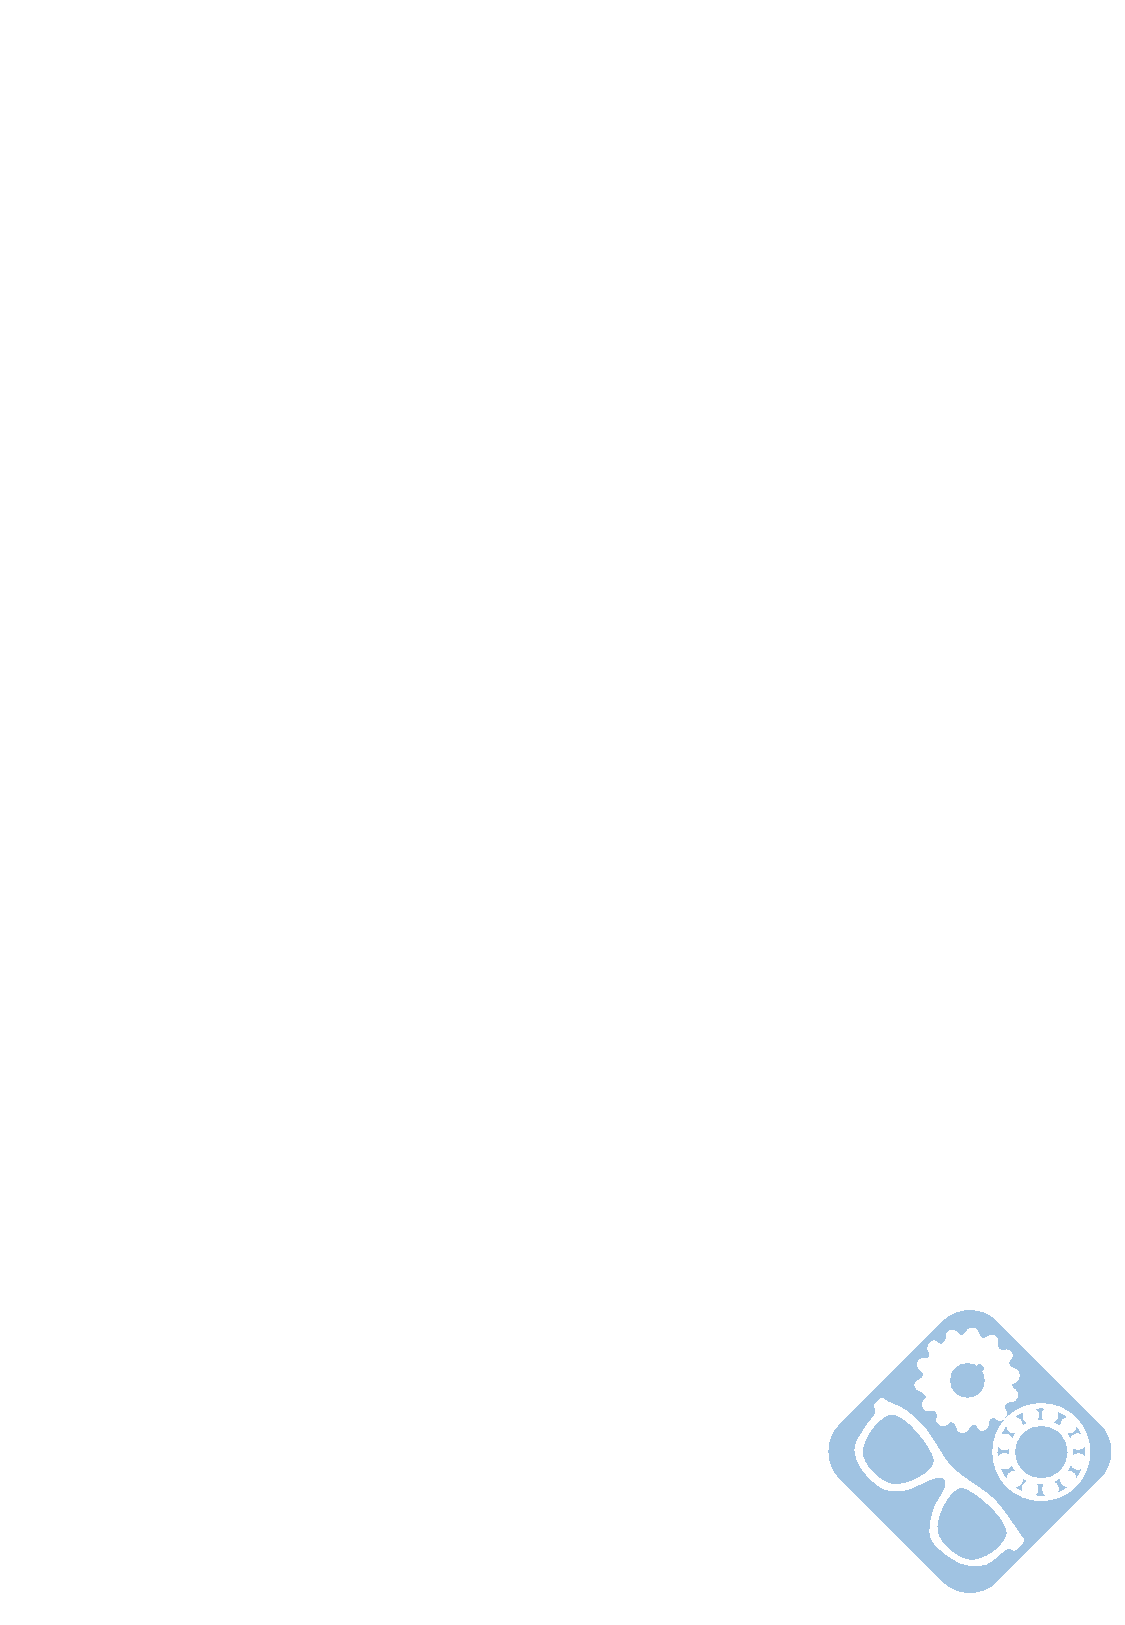
\includegraphics[width=\paperwidth,height=\paperheight,%
keepaspectratio]{../../../img/fond4}%
\end{center}
\vfill
}}}

\begin{document}

\pagestyle{empty}

\AddToShipoutPicture*{\BackgroundPic}


\includegraphics[width=2cm]{../../../img/logo}

\Huge{DS \numero - \sujet}

\vspace{1cm}

\ifdef{\prive}{\begin{center}\colorbox{danger}{\Huge{Avec Correction}}\end{center}}{}

\begin{center}
\centering\huge{PTSI}
\end{center}

\vspace{2cm}


\begin{center}
\centering\Large{\jour}
\end{center}

\vspace{2cm}

\normalsize

\tableofcontents

\newpage

\AddToShipoutPicture{\BackgroundPicdeux}

\pagestyle{fancy}

\begin{center}
\Huge \sujet
\end{center}


\normalsize


\section{Présentation}

Les constructeurs automobiles sont sans cesse dans l'obligation d'innover pour rester attractifs vis-à-vis du client. Les ouvrants pilotés automobiles font partie des atouts différenciateurs. Le terme ouvrant désigne à la fois les lève-vitres électriques, les toits ouvrants, les toits escamotables, les coffres motorisés et les portes latérales coulissantes. Tous ces ouvrants sont une source d'attrait pour le client, de par leur praticité ou encore par leurs facteurs de différenciation importants. 

\begin{figure}[!h]
\centering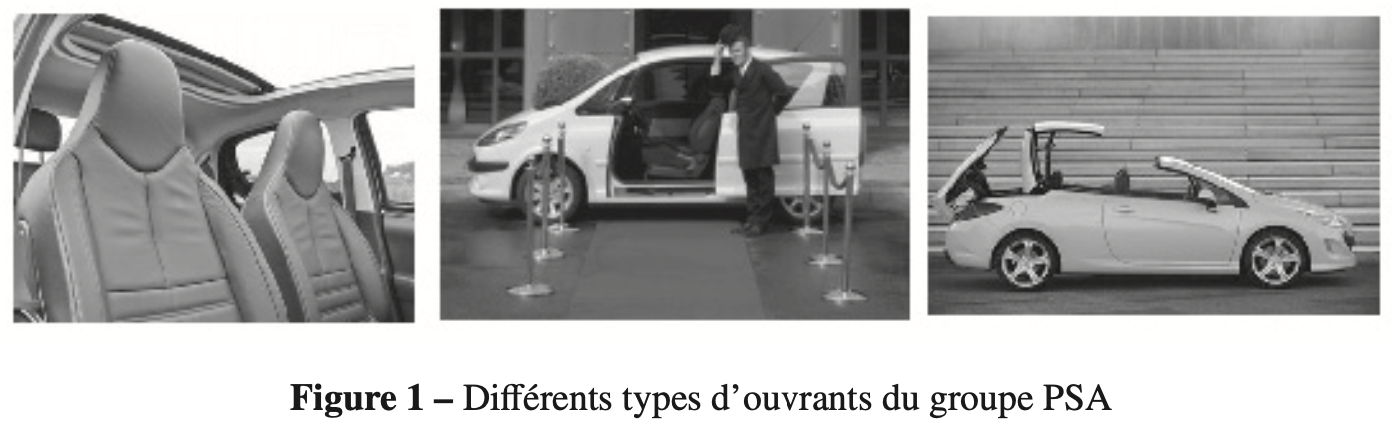
\includegraphics[width=0.65\linewidth]{img/figure01}
 \caption{Poudre de maquillage compactée avant et après création des motifs}
 \label{img01}
\end{figure}

Il existe deux types de pilotage des ouvrants : 
\begin{itemize}
 \item le premier est un système classique et/ou d'assistance. L'utilisateur gère complètement le déplacement de l'ouvrant. Dès qu'il arrête son action sur la commande, l'ouvrant s'immobilise, c'est le cas par exemple du lève-vitre électrique non séquentiel. Ainsi, avec un système classique et/ou d'assistance, le déplacement de l'ouvrant est entièrement imputable aux actions de l'utilisateur ; 
 \item le second type est le pilotage automatisé des ouvrants. Ici, l'utilisateur demande simplement à ce que l'ouvrant se déplace jusqu'à une position prédéfinie. Une brève action de sa part entraîne le déplacement complet de l'ouvrant. Pour le lève-vitre électrique séquentiel, l'utilisateur demande à ce que la vitre remonte complètement, par une courte action sur l'interrupteur. Dès lors, le système de contrôle/commande gère le déplacement de l'ouvrant dans le cas normal, mais aussi en cas de dysfonctionnement (perte de fonctionnalité ou présence d'un obstacle sur le trajet de la vitre). Il faut donc assurer un fonctionnement sûr et robuste du système d'ouvrant piloté automatisé pour éviter que le système blesse un occupant. 
\end{itemize}

\begin{figure}[!h]
\centering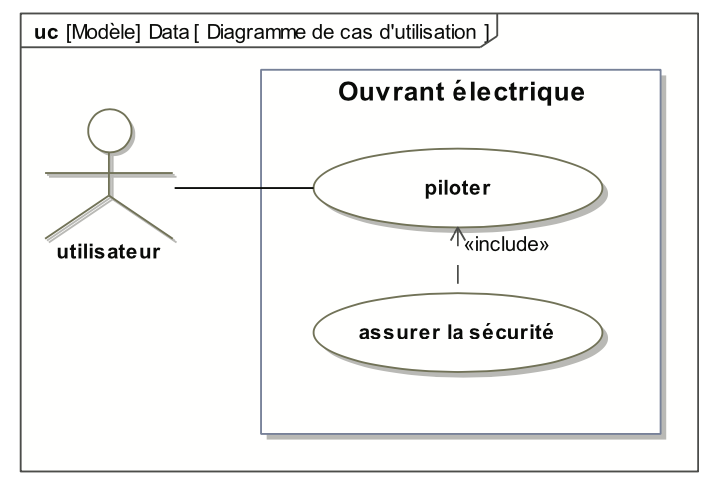
\includegraphics[width=0.35\linewidth]{img/figure02}
 \caption{Diagramme des cas d'utilisation d'un ouvrant électrique}
 \label{img02}
\end{figure}

Le diagramme de cas d'utilisation de la figure \ref{img02} synthétise les explications précédentes. 

\paragraph{Objectif:}

L'objectif du travail proposé dans ce sujet est de mettre en place différentes stratégies de commande d'un lève-vitre électrique de Peugeot 308 de manière à pouvoir extrapoler les résultats à une porte coulissante électrique. Cette étude nécessite : 
\begin{itemize}
 \item une analyse de l'architecture du lève-vitre (partie I) ;
 \item une modélisation multiphysique du système (partie II) ;
 \item le développement d'un modèle de commande de type asservissement continu (partie III).
\end{itemize}

\begin{figure}[!h]
\centering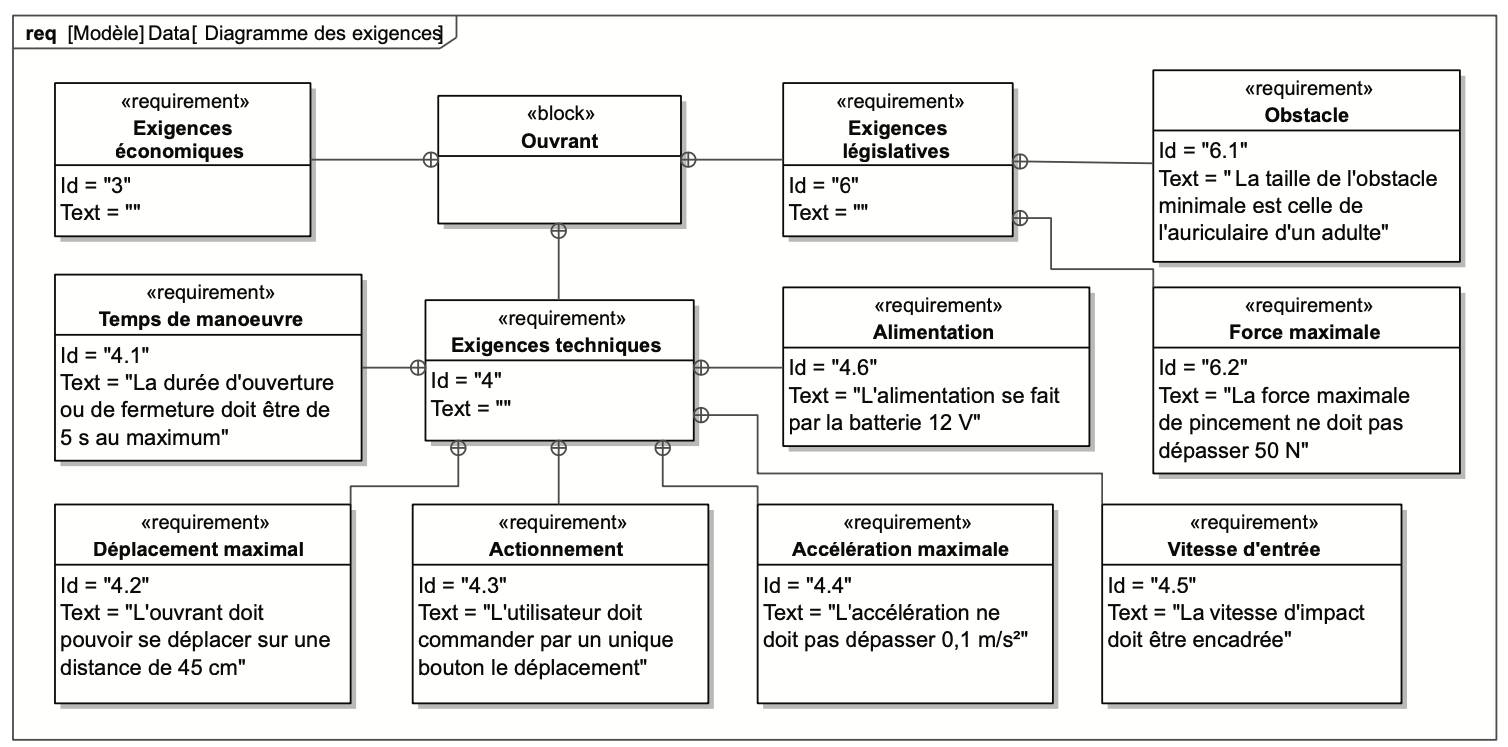
\includegraphics[width=0.85\linewidth]{img/figure03}
 \caption{Diagramme des cas d'utilisation d'un ouvrant électrique}
 \label{img03}
\end{figure}
 
Le diagramme des exigences de la figure \ref{img03} liste quelques performances attendues pour le lève-vitre électrique. 

\section{Architecture du lève-vitre}

Pour le développement et la mise en œuvre d'une architecture de commande, il est nécessaire de disposer d'un modèle de simulation fiable et précis, tout en connaissant ses limites de validité. 

L'élaboration d'un tel modèle nécessite de décrire l'implantation de la chaîne d'énergie et de la chaîne d'informations de l'ouvrant. 
Le diagramme de définitions de blocs de la figure \ref{img04}, page suivante, liste l'ensemble des constituants principaux du lève-vitre électrique. La plupart des constituants sont repérés sur la figure \ref{annexe}. 

\question{Compléter, à l'aide des noms disponibles sur le diagramme de la figure \ref{img04}, le schéma des chaînes fonctionnelles du document réponse.}

~\

Le réducteur du lève-vitre est constitué d'un dispositif roue et vis sans fin. La roue possède $Z =53$ dents et la vis est constituée d'un seul filet, figure \ref{annexe}.  Le câble s'enroule sur le tambour de diamètre $D=41.5\ mm$, solidaire de la roue. Le câble est solidaire du coulisseau sur lequel est fixée la vitre. 

\begin{figure}[!h]
\centering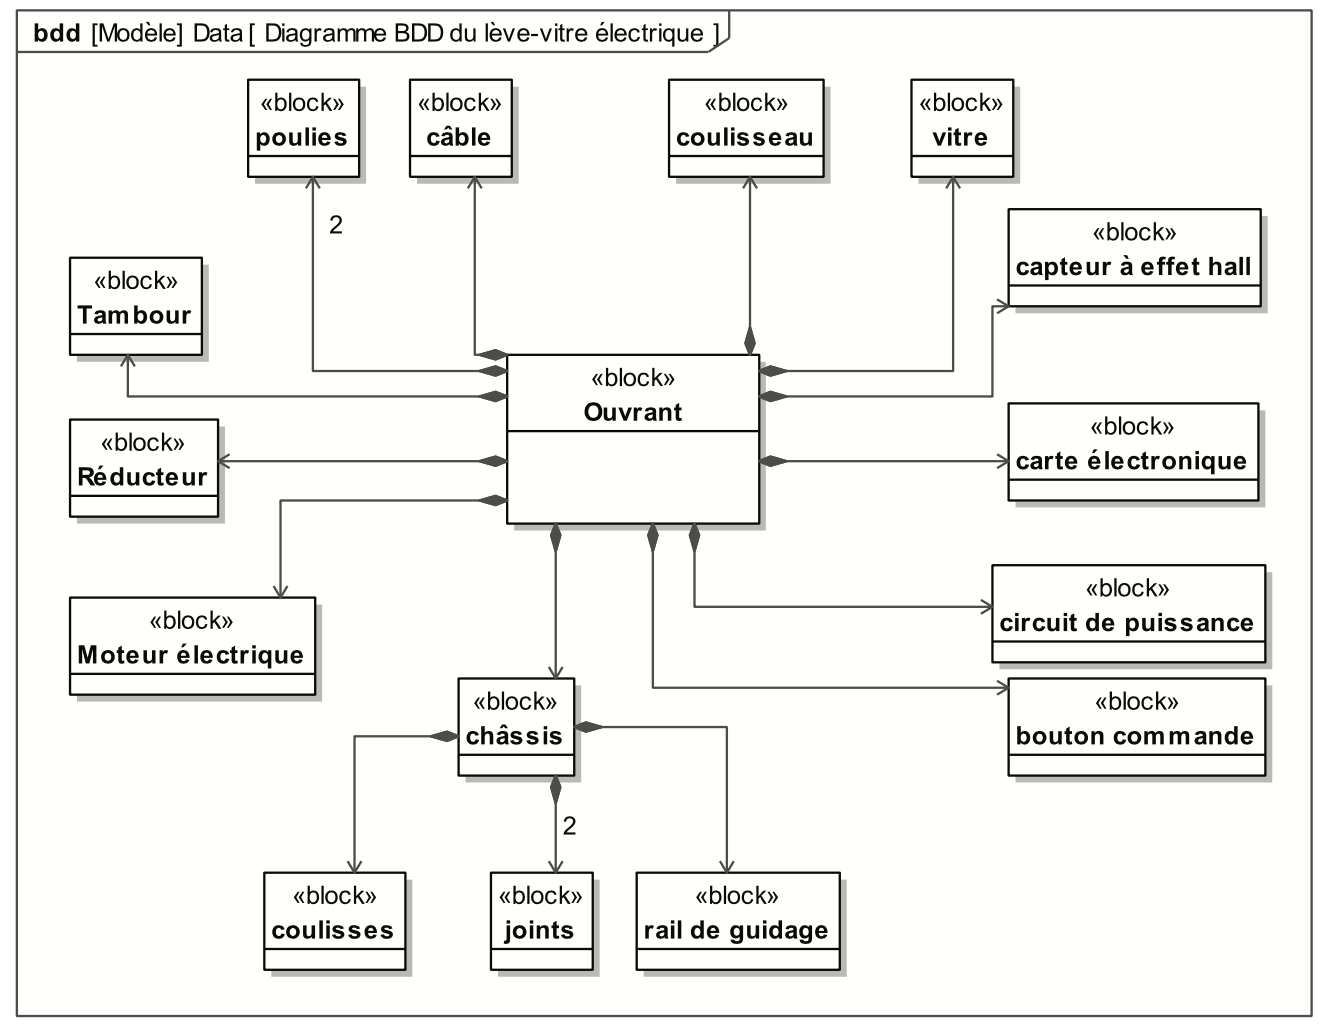
\includegraphics[width=0.75\linewidth]{img/figure04}
 \caption{Diagramme de définition de blocs (BDD) du lève vitre électrique}
 \label{img04}
\end{figure}

On note $v(t)$ la vitesse de déplacement en translation de la vitre et $\omega_m(t)$ la vitesse angulaire du moteur.

\question{Déterminer l'expression littérale du rapport de réduction r (roue et vis + poulie) tel que $v(t)=r \cdot \omega_m(t)$. Effectuer l'application numérique.}

Quelque soit le résultat trouvé précédemment, on prendra $r=0,39\ mm.rad^{-1}$.

\question{Déterminer le nombre de tours $n_m$ que doit faire le moteur pour obtenir le déplacement de la vitre indiqué dans le diagramme des exigences.}

\question{Sachant que le régime nominal du moteur est de $N_m=4000$ tours/minute, en déduire la durée (en s) d'ouverture/fermeture de la fenêtre. Conclure quant à l'exigence correspondante du diagramme des exigences.}

\section{Modélisation multiphysique du système}

Un modèle multiphysique doit être mis en place pour pouvoir prendre en compte tous les phénomènes qui apparaissent lors du fonctionnement de la vitre sans et avec obstacle.

\begin{figure}[!h]
\centering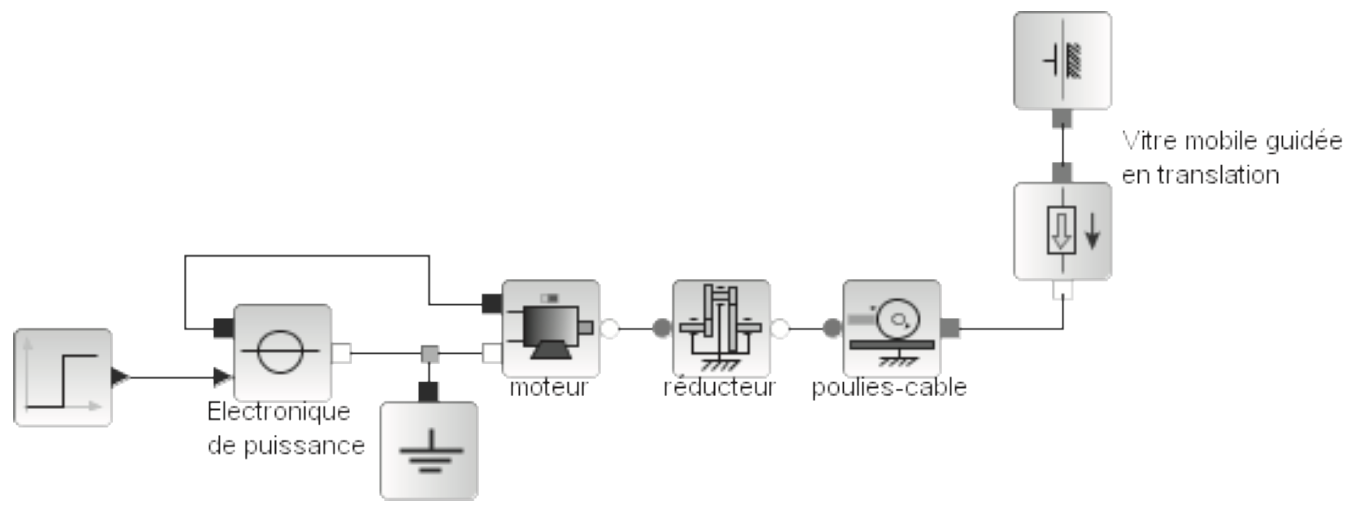
\includegraphics[width=0.85\linewidth]{img/figure05}
 \caption{Modélisation multi-physique du lèvre vitre sans obstacle}
 \label{img05}
\end{figure}

Les différents éléments intervenant dans ce modèle doivent être caractérisés séparément pour obtenir une représentation la plus fidèle possible de la réalité. 

\question{Indiquer sur quel bloc paramétrer la résistance et l'inductance interne du moteur.}

Les deux questions suivantes sont à réaliser sur le document réponse.

\question{Colorier en bleu/vert les fils sur lesquels circule une énergie électrique/mécanique.}

\question{On souhaite ajouter un bloc permettant de modéliser les frottements mécaniques de la vitre sur le joint de la porte. Proposer en indiquant une croix un emplacement pour ce bloc.}

\subsection{Guidage d'une porte coulissante}

\begin{figure}[!h]
\begin{minipage}{0.5\linewidth}
La structure de la porte coulissante électrique est proche de celle du lève-vitre (figure \ref{img08}).

Un moto-réducteur entraîne, par l'intermédiaire
d'un tambour et de poulies/câble, la porte qui est guidée par trois rails (inférieur, milieu et supérieur) grâce à trois chariots en liaison avec la porte.

Des galets (trois par chariot) sont montés sur ces chariots pour assurer le guidage avec les rails.

La chaîne d'information de la porte coulissante est exactement la même que pour le lève- vitre.

Le diagramme BDD de la porte coulissante est donné sur la figure \ref{img09}. 

\end{minipage}\hfill
\begin{minipage}{0.45\linewidth}
\centering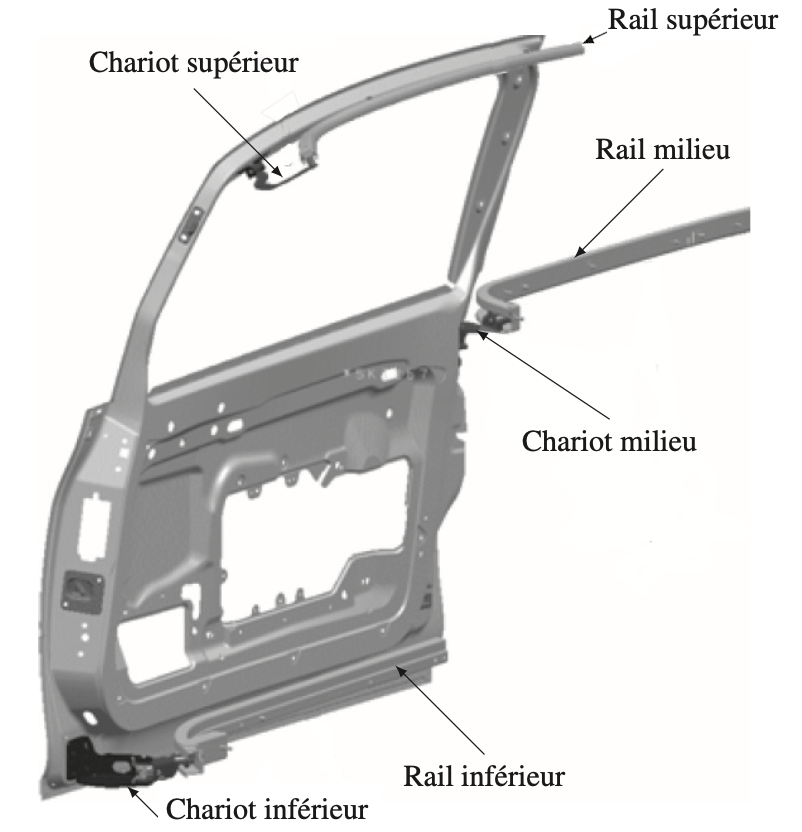
\includegraphics[width=0.7\linewidth]{img/figure08}
 \caption{Description du système de guidage de la porte coulissante électrique}
 \label{img08}
\end{minipage}
\end{figure}

\question{En comparant les diagrammes BDD de la porte coulissante et de la vitre, indiquer de manière synthétique les sous-ensembles qui diffèrent (ne pas lister tous les constituants).}

\question{Indiquer d'après vous l'intérêt de la solution de guidage retenue pour la porte coulissante par rapport à celle du lève-vitre.}

\begin{figure}[!h]
\centering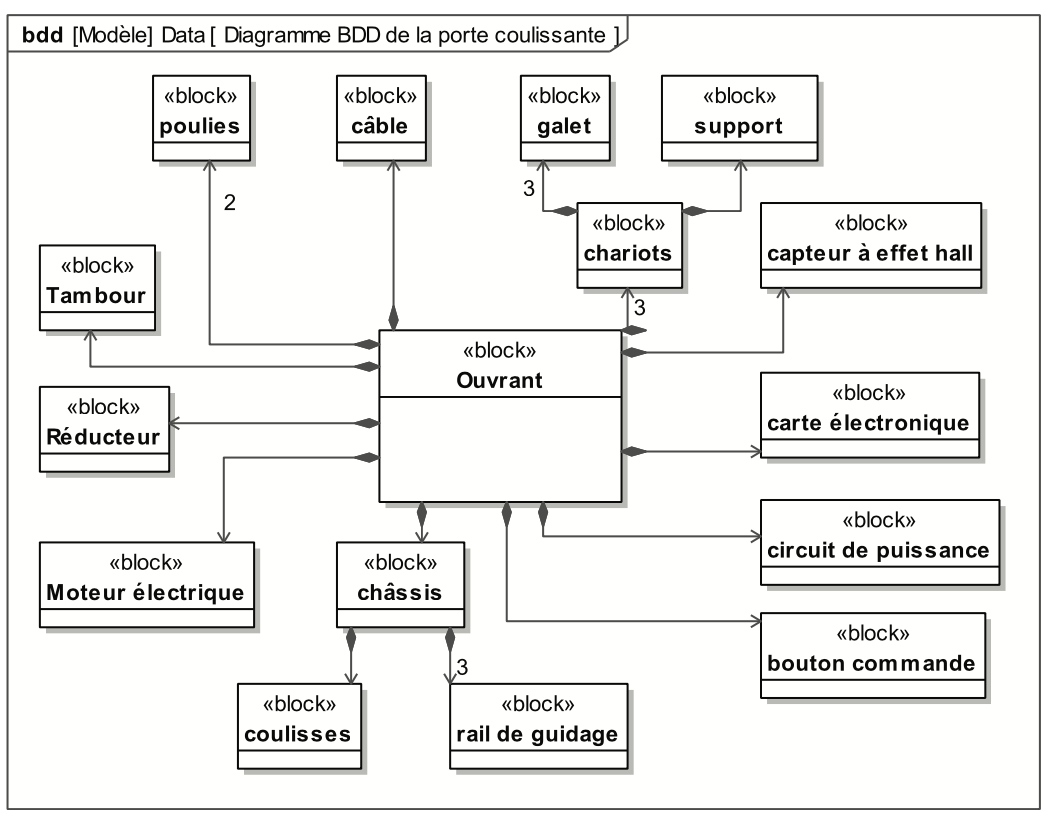
\includegraphics[width=0.6\linewidth]{img/figure09}
 \caption{Diagramme BDD de la porte coulissante}
 \label{img09}
\end{figure}

\newpage

\subsection{Validation du modèle simplifié}

La simulation de la figure \ref{img11} compare l'évolution de la position de la vitre et de la vitesse du moteur selon trois cas sans obstacle : sans effort résistant, pour un effort résistant constant moyen et pour un effort résistant variable en fonction de la position de la vitre. 

\begin{figure}[!h]
\centering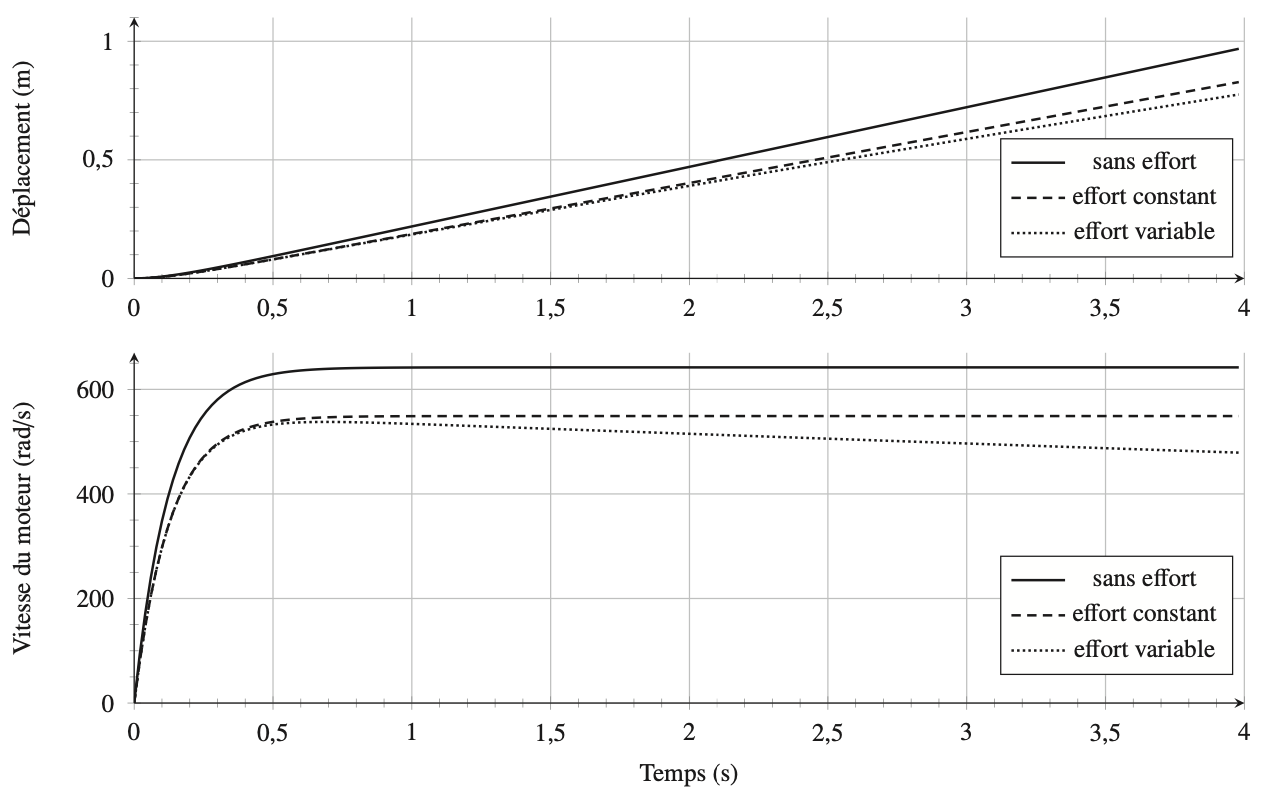
\includegraphics[width=0.75\linewidth]{img/figure11}
 \caption{Courbe de la position de la vitre et de la vitesse de rotation du moteur}
 \label{img11}
\end{figure}

\question{Dans chacune des situations, relever le temps au bout duquel la vitre atteint la position maximale définie dans le diagramme des exigences. Commenter l'influence de l'effort résistant sur la vitesse en régime permanent et en régime transitoire. Justifier votre choix entre un modèle sans effort résistant et un modèle avec prise en compte de l'effort résistant.}

~\

Pour détecter un pincement, une solution envisagée est d'utiliser le courant dans le moteur et de repérer une variation de ce courant. La simulation multiphysique permet de calculer le courant dans le moteur dans le cas de la présence d'un obstacle ou non.

Les courbes de la figure \ref{img12} ont été obtenues en prenant une raideur d'obstacle de 20 N/mm et correspondent à la position de la vitre en m, à l'intensité du moteur en A et à l'effort de pincement en N. 

\begin{figure}[!h]
\centering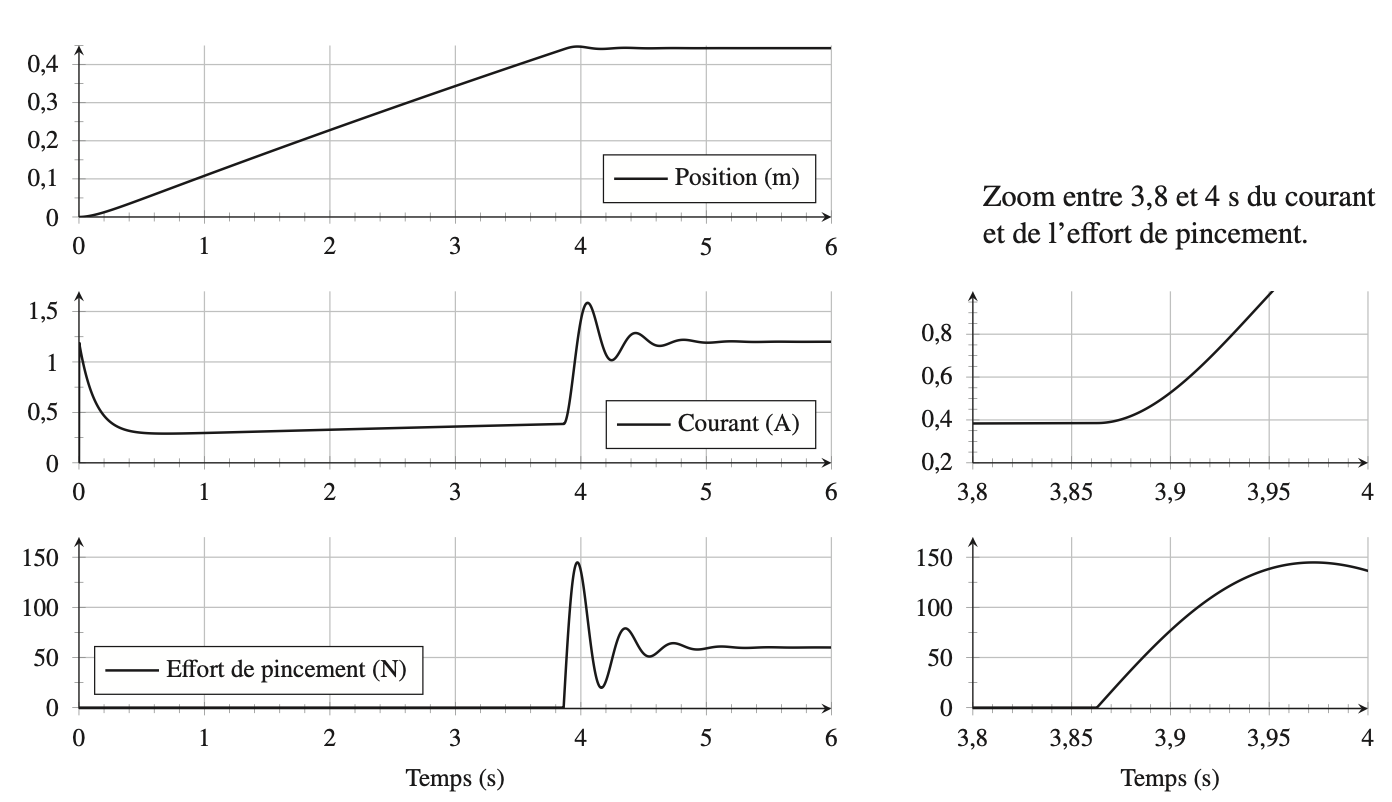
\includegraphics[width=0.8\linewidth]{img/figure12}
 \caption{Courbe de position de la vitre, d'intensité moteur et d'effort de pincement}
 \label{img12}
\end{figure}

\question{Déterminer l'intervalle de temps où l'effort est inférieur à la force maximale admissible donnée par la législation (diagramme des exigences de la figure \ref{img03}). En déduire la variation de courant sur cet intervalle et la comparer à celle obtenue au démarrage. Conclure sur la fiabilité de la mesure de courant pour repérer précisément un obstacle.}

\section{Commande asservie}

Il est nécessaire de prendre en compte une commande asservie de vitesse lors de détection de  pincement; c'est le cas de la porte coulissante où la vitesse est variable et contrôlée selon les moments de fonctionnement. 

\subsection{Mise en place de l'asservissement de vitesse}

On considère la vitre de masse m se déplaçant verticalement. Le moment d'inertie du rotor autour de son axe de rotation est noté $J_m$. Les inertie, autres que celles de la vitre et du rotor, sont négligées.

On appelle $\omega_m(t)$ la vitesse angulaire du moteur et r le rapport de réduction entre la vitesse $v(t)$ de la vitre et la vitesse angulaire du moteur $v(t)=r.\omega_m(t)$.

Le référentiel lié à la voiture est supposé galiléen.

On pose:
\begin{itemize}
 \item $f_v$ le coefficient de frottements visqueux de l'axe moteur,
 \item $C_r(t)$ le couple résistant ramené au niveau de l'arbre moteur. celui-ci prend en compte les frottements (autres que ceux dans le moteur), la pesanteur et aussi la présence ou non d'obstacle; ce sont les seules pertes. Toutes les autres liaisons sont considérées comme parfaites,
 \item $C_m(t)$ le couple exercé par le moteur,
 \item $k_e$ la constante électrique du moteur,
 \item $R_m$ la résistance de l'induit du moteur,
 \item $k_c$ la constante de couple. 
\end{itemize}

On donne l'équation suivante: $J\cdot \frac{d\omega_m(t)}{dt}+f_v\ \omega_m(t)=C_m(t)-C_r(t)$

\question{Écrire les 3 autres équations du moteur à courant continu.}

\question{Montrer que $\left [\frac{\Omega_m(p)}{U_m(p)}    \right]_{C_r(p)=0}=\frac{K_m}{1+\tau_m\cdot p}$}

L'asservissement en vitesse est obtenu grâce à un capteur placé sur le rotor du moteur, de gain $K_{capt}$. Ce capteur délivre une tension qui est ensuite comparée à une tension de consigne image de la consigne de vitesse $\omega_c(t)$ par un gain d'adaptation de même valeur. On utiliser un correcteur/amplificateur de fonction de transfert $C_{corr}(p)$ qui fournit la tension $u_m(t)$ au moteur à partir de l'écart $\varepsilon_u(t)$.

La figure suivante présente le schéma bloc de l'asservissement avec 2 entrées $\Omega_c(p)$ et $C_r(p)$ (respectivement la vitesse angulaire de consigne du moteur et le couple résistant) et une sortie $\Omega_m(p)$.

\begin{figure}[!h]
\centering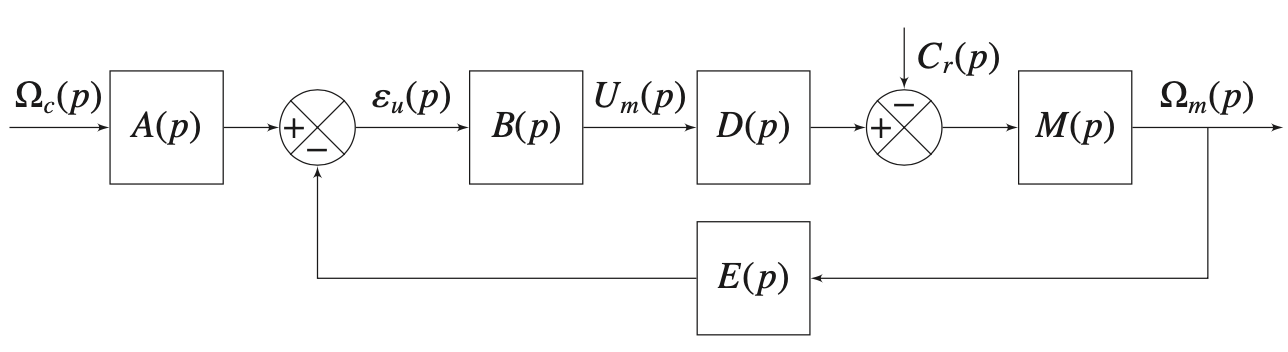
\includegraphics[width=0.55\linewidth]{img/figure15}
 \caption{Schéma-bloc équivalent de l'asservissement de vitesse du moteur}
 \label{img15}
\end{figure}

\question{Déterminer l'expression de $A(p)$ pour avoir $\varepsilon_u(p)=0$, image de $\Omega_m(p)-\Omega_c(p)$.}

\question{Déterminer les expressions des fonctions A(p), B(p), D(p), M(p) et E(p) intervenant dans ce schéma à partir des données de l'énoncé.}

\begin{figure}[!h]
\centering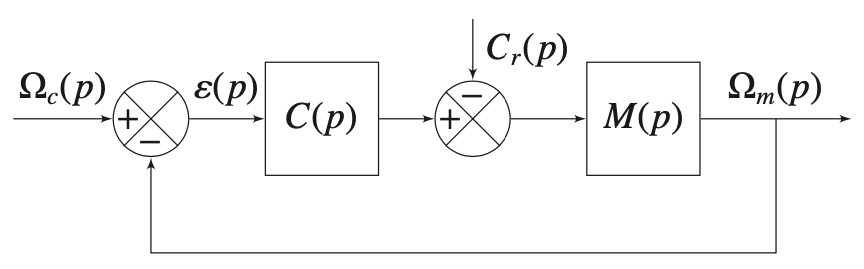
\includegraphics[width=0.4\linewidth]{img/figure16}
 \caption{Schéma-bloc équivalent de l'asservissement de vitesse du moteur}
 \label{img16}
\end{figure}

Le schéma-blocs de la figure \ref{img16} est un schéma-blocs équivalent au schéma de la figure \ref{img15}.

\question{Déterminer l'expression de la fonction de transfert C(p) en fonction de $k$, $r$, $C_{corr}(p)$ et $K_{capt}$.}

\question{Déterminer l'expression de $\Omega_m(p)=H_1(p) \cdot \Omega_c(p) + H_2(p) \cdot  C_r(p)$ où on donnera les expressions de $H_1(p)$ et $H_2(p)$ en fonction des fonctions de transfert $M(p)$ et $C(p)$. Pour information: $H_1(p)=\left [\frac{\Omega_m(p)}{\Omega_c(p)} \right ]_{C_r(p)=0}$ et $H_2(p)=\left [\frac{\Omega_m(p)}{C_r(p)} \right ]_{\Omega_c(p)=0}$}

~\

Dans la suite du sujet, on prendra la fonction $M(p)=\frac{K}{1+\tau\ p}$ avec $K=53,5\ rad.s^{-1}$ et $\tau=0,13\ s$.

\question{Exprimer $\varepsilon(p)$ en fonction de $\Omega_c(p)$ et $C_r(p)$ sous la forme $\varepsilon(p)=H_c(p)\cdot\Omega_c(p)+H_r(p)\cdot C_r(p)$ où on donnera les expressions de $H_c(p)$ et $H_r(p)$ en fonction des fonctions de transfert $M(p)$ et $C(p)$.}

\subsection{Vérification des performances de l'asservissement de vitesse}

Compte-tenu des études menées précédemment $\Omega_c(p)$ peut être modélisée par un échelon ou une rampe, de même pour $C_r(p)$.

On commence par utiliser un correcteur proportionnel $C(p)=K_p=0.6$, et $C_r(p)=0$.

\question{Exprimer la fonction de transfert boucle fermée du système $H_1(p)$, sous forme canonique, en fonction de $K$, $K_p$ et $\tau$. Préciser l’ordre et la classe de ce système.}

\question{Déterminer l’équation de la réponse temporelle $\omega_m(t)$ à une entrée en échelon $\omega_c(t)=1 rad.s^{-1}$.}

\question{Tracer sur le document réponse la réponse temporelle $\omega_m(t)$ en indiquant toutes les valeurs caractéristiques connues. Vous ferez apparaître l’entrée en échelon. Compléter les axes afin de faire apparaître les valeurs des graduations principales en abscisse et ordonnée.}

\question{Calculer alors l’erreur statique notée $\varepsilon_s$ en fonction de $K_p$ et $K$. Conclure sur la précision du système avec ce type de correcteur.}

\question{Sur le document réponse, tracer le diagramme asymptotique de la fonction de transfert $H_1(p)$ (vous indiquerez clairement les pentes en dB/décades et les valeurs de phase des asymptotes. Compléter les axes afin de faire apparaître les valeurs des graduations principales en abscisse et ordonnée.}

~\

On choisit maintenant d’utiliser un correcteur proportionnel intégral. Ainsi, la fonction de transfert équivalente C(p) peut s’écrire $C(p)=K_p\frac{1+\tau_i\cdot p}{\tau_i\cdot p}$.

\question{Exprimer la fonction de transfert boucle fermée du système $H_1(p)$, sous forme canonique, en fonction de $K$, $K_p$, $\tau$ et $\tau_i$. Préciser l’ordre et la classe de ce système.}

\question{Calculer l’erreur statique notée $\varepsilon_{s1}$ pour $C_r(p)=0$ et $\Omega_c(p)=\frac{\Omega_{c0}}{p}$ où $\Omega_{c0}=1.$}

\question{Calculer l’erreur statique notée $\varepsilon_{s2}$ pour $\Omega_c(p)=0$ et $C_r(p)=\frac{C_{r0}}{p}$ où $C_{r0}$ est une constante.}

\question{Calculer l’erreur de traînage en régulation notée $\varepsilon_{t1}$ pour $C_r(p)=0$ et $\Omega_c(p)=\frac{a}{p^2}$ où $a$ est une constante.} 

\question{Calculer l’erreur de traînage en régulation notée $\varepsilon_{t2}$ pour $\Omega_c(p)=0$ et $C_r(p)=\frac{b}{p^2}$ où $b$ est une constante.} 

~\

Si un obstacle apparaît, le couple résistant est donné par $Cr(p) = C_{obs}(p) + C_{nom}(p)$ avec $C_{obs}(p)$ le couple résistant ramené sur l’axe moteur dû à l’obstacle et $C_{nom}(p)$ les autres couples résistants (frottements, pesanteur).

Pour détecter l’apparition d’un obstacle, on détermine une approximation du couple $C_{obs}(p)$. Pour ce faire, on suppose que l’erreur due à la perturbation s’écrit sous la forme suivante : 
$\varepsilon(p) = \varepsilon_{t2} + H_r(p)C_{obs}(p)$ avec  l’erreur de traînage en régulation constante déterminée à la question précédente.

Étant donné que l’on souhaite détecter rapidement la variation anormale de couple, on approche $Hr(p)$ par son comportement à haute fréquence. 

En prenant les valeurs suivantes pour $K_p=0,6$ et $\tau_i=10 \cdot \tau$, on obtient après calcul la fonction $H_r(p)=\frac{2,2\;p}{(1+1,34p)(1+0,004p)}$.

\question{Tracer sur le document réponse les diagrammes de Bode asymptotiques de la fonction $H'_r(p)=\frac{H_r(p)}{p}=\frac{2,2}{(1+1,34p)(1+0,004p)}$ en justifiant les pulsations de coupure. Compléter les axes afin de faire apparaître les valeurs des graduations principales en abscisse et ordonnée.}

\question{Tracer sur le document réponse les diagrammes de Bode asymptotiques de la fonction $H_r(p)$ en justifiant les pulsations de coupure. Compléter les axes afin de faire apparaître les valeurs des graduations principales en abscisse et ordonnée.}

\question{En utilisant l’expression de la fonction de transfert $H_r(p)$ ou les diagrammes de Bode, proposer une approximation de $H_r(p)$ pour des pulsations supérieures à $100 rad.s^{-1}$. En déduire l’expression de $C_{obs}(p)$ approchée, en fonction de $\varepsilon$, $\varepsilon_{t2}$, $K$ et $\tau$ à partir de l’expression de $\varepsilon$ obtenue à la question précédente.}

~\

Les réglages du correcteur proportionnel intégral permettent d’obtenir un système asservi rapide et stable.

Une simulation est réalisée pour une consigne de vitesse angulaire $\omega_c$ variable pendant laquelle un obstacle apparaît à un instant donné avant la fermeture complète de la vitre. Les évolutions de la vitesse du moteur, de la position de la vitre, du couple résistant et du couple estimé $C_{obs}$ sont tracées sur la figure \ref{img17}.

\begin{figure}[!h]
\centering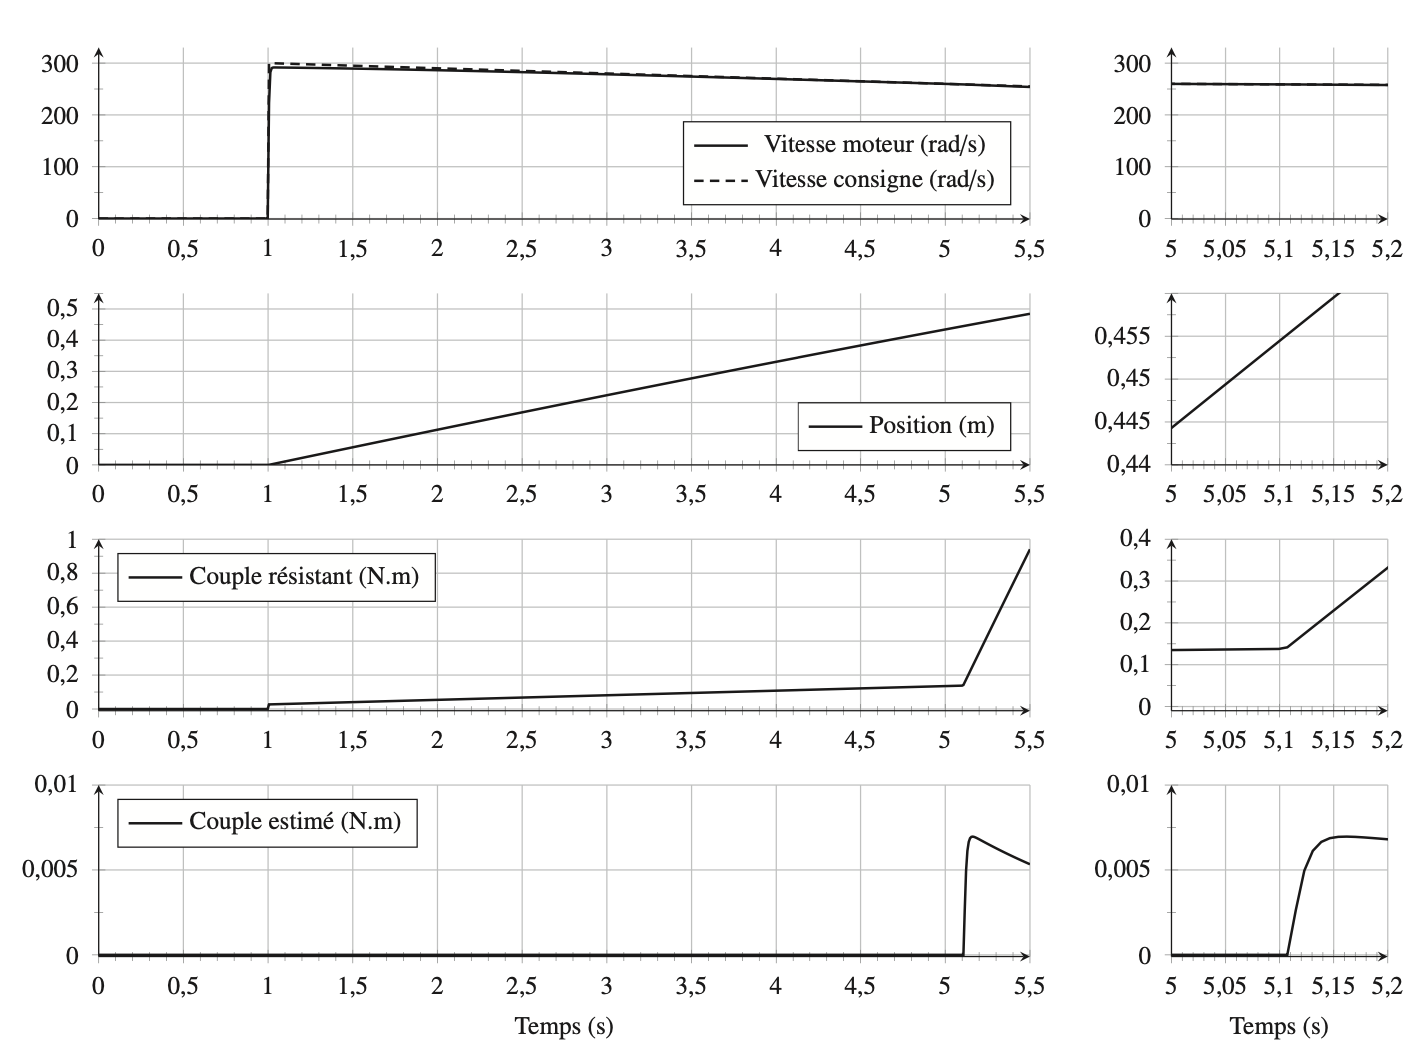
\includegraphics[width=0.8\linewidth]{img/figure17}
 \caption{Courbes de vitesse et de position, courbes du couple résistant et du couple généré par l'obstacle estimé (zoom entre 5 et 5,2 s à droite)}
 \label{img17}
\end{figure}

\question{Indiquer à quel instant l’obstacle intervient et expliquer qualitativement comment utiliser l’estimation de $C_{obs}$ pour repérer un obstacle.}

\section{Identification à partir d'un diagramme de Bode}

Soit le diagramme de Bode suivant.

\begin{figure}[!h]
\centering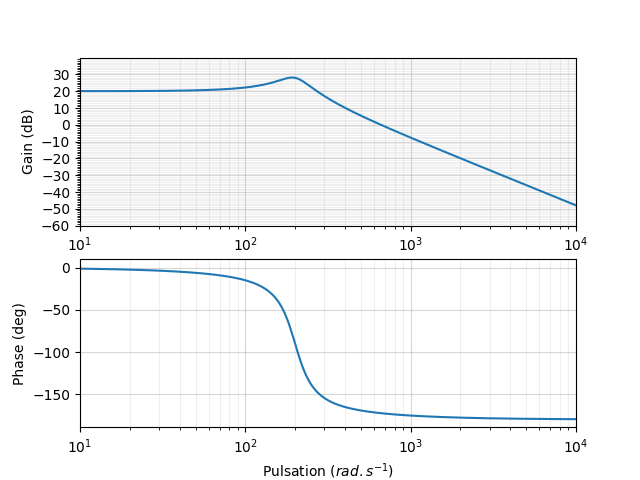
\includegraphics[width=0.85\linewidth]{img/Q33}
 \caption{Diagramme de Bode de la fonction de transfert à identifier}
 \label{img18}
\end{figure}

\question{Identifier la fonction de transfert dont le diagramme de Bode est présenté à la figure \ref{img18}. Justifier les réponses.}

\newpage

\section{Annexe}

\begin{figure}[!h]
\centering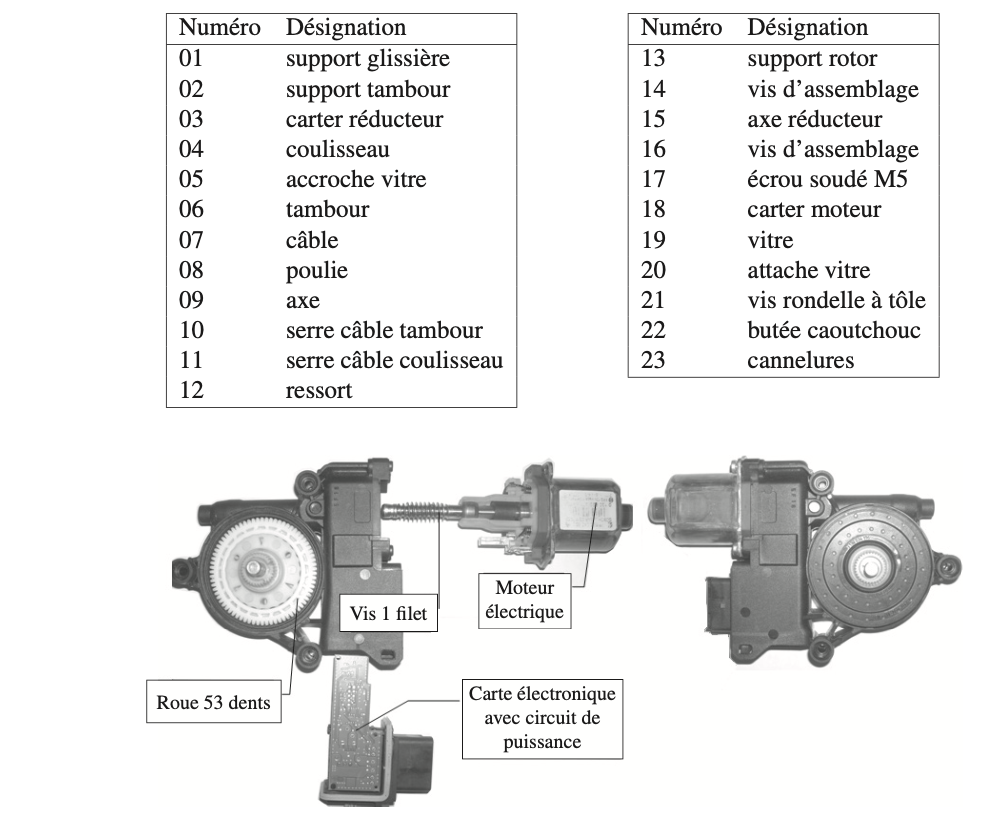
\includegraphics[width=0.85\linewidth]{img/annexe} \caption{Éclaté du motoréducteur}
 \label{annexe}
\end{figure}

\cleardoublepage

\ifdef{\public}{\pagestyle{documentreponse}}{\pagestyle{correction}}

\reponse{0}{\begin{center}
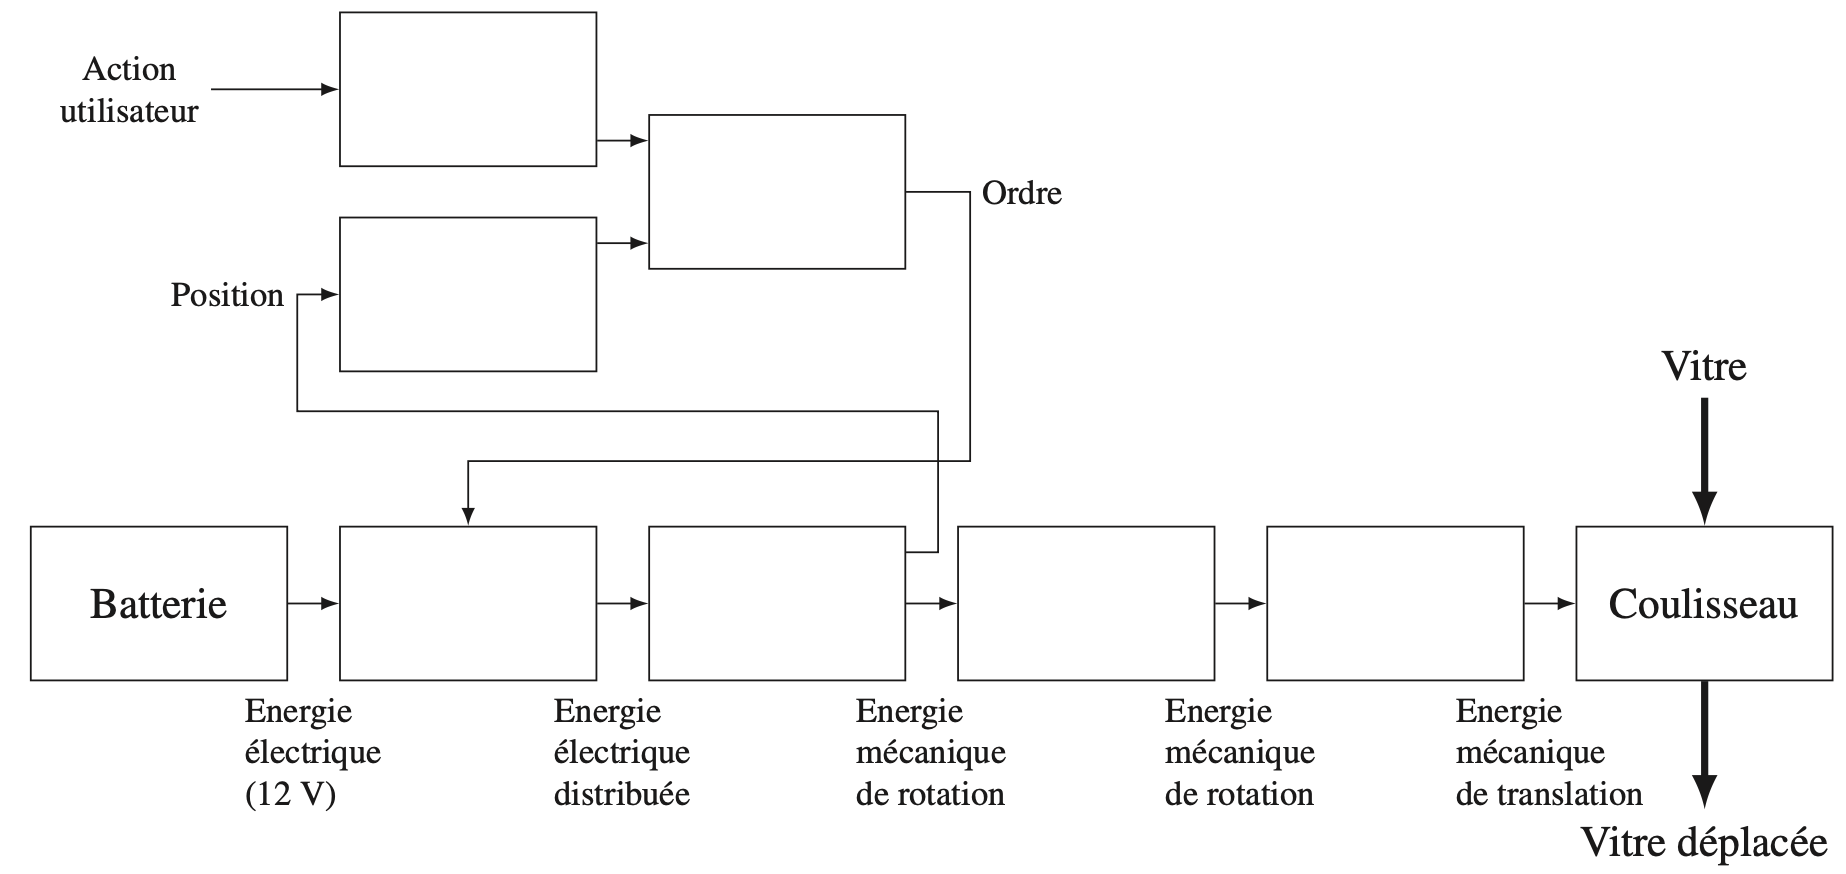
\includegraphics[width=0.8\linewidth]{img/DR01}
\end{center}}{
\begin{center}
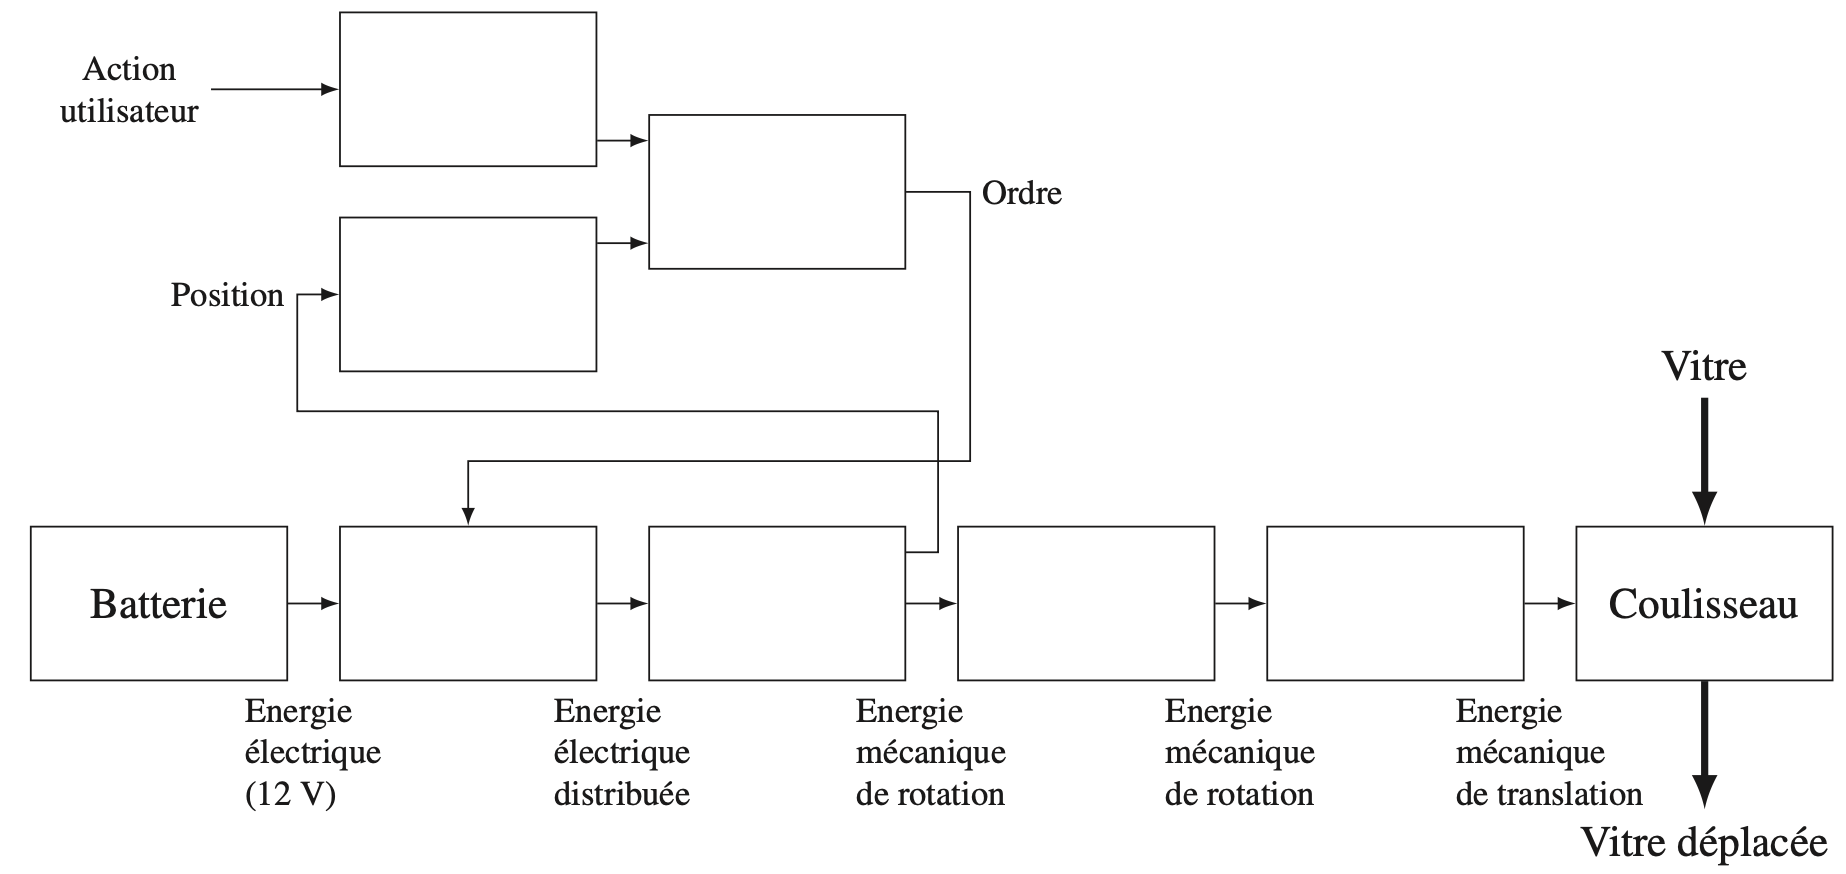
\includegraphics[width=0.8\linewidth]{img/DR01_cor}
\end{center}}

\vspace{-1cm}

\reponse{4}{}{
$v(t)=\frac{D}{2}\cdot\omega_p(t)=\frac{D}{2}\cdot\frac{1}{Z}\cdot\omega_m(t)$

$v(t)=20.75\cdot\frac{1}{53}\cdot\omega_m(t)=0.39\cdot\omega_m(t)$

$r=\frac{D}{2\cdot Z}$ avec $r=0.39mm$.}

\reponse{3}{}{
La distance à parcourir est de $45cm$ (req 4.2). L'angle moteur est donc donné par $\theta_m=\frac{450}{r}=\frac{450}{0.39}=1154rad$, on en déduit $n_m=182tours$.}

\reponse{3}{}{
À vitesse nominale on a $T=\frac{n_m}{N_m}=\frac{182}{4000}=0.045min=2.7s$. Cette durée est inférieure aux 5 secondes fixées par l'exigence 4.1 du cahier des charges. }

\reponse{2}{}{
Il faut indiquer cette valeur dans le bloc moteur.}

\reponse{0}{Répondre dans la case suivante.}{Réponse dans la case suivante.}

\reponse{0}{\begin{center}
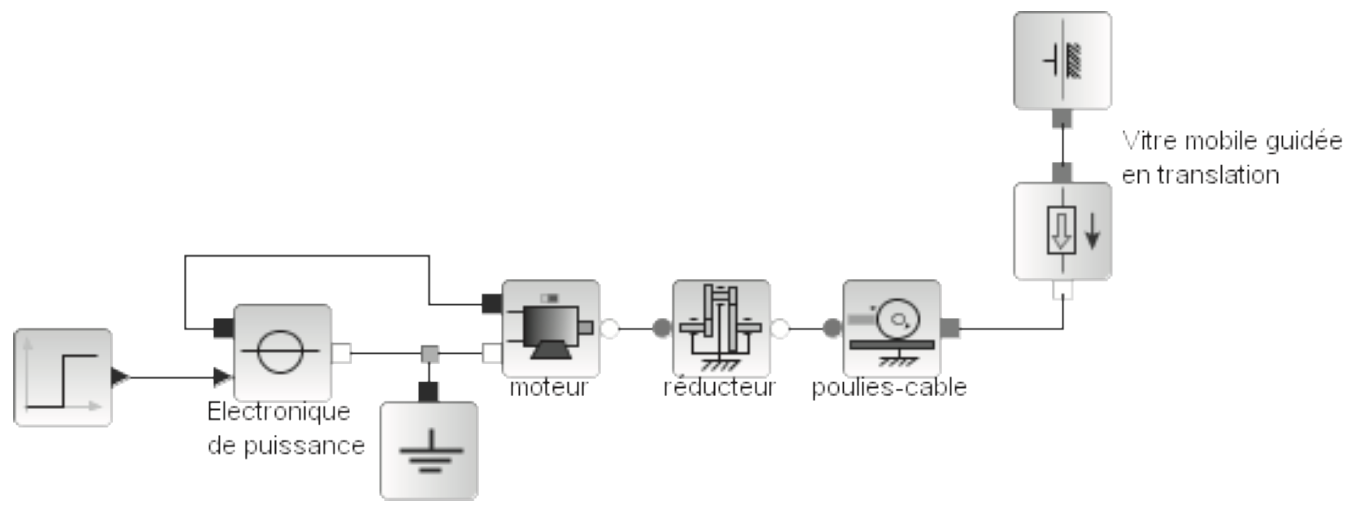
\includegraphics[width=0.9\linewidth]{img/figure05}
\end{center}}{
\begin{center}
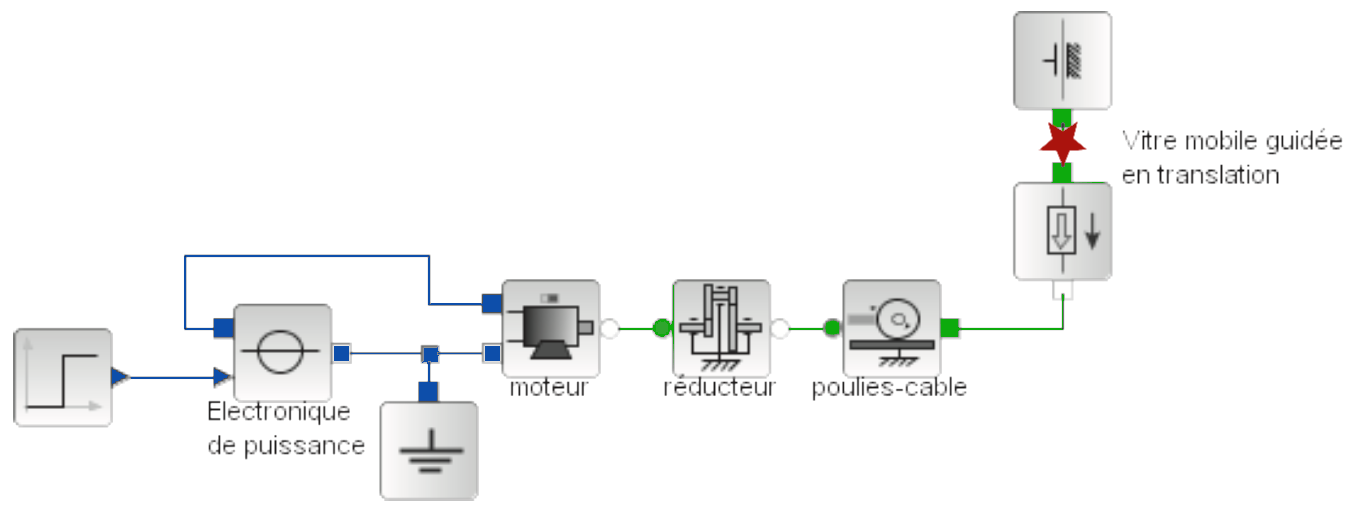
\includegraphics[width=0.9\linewidth]{img/figure05_cor}
\end{center}}

\reponse{2}{}{Les éléments qui diffèrent sont les joints ainsi que les blocs coulisseaux et supports \og remplacés \fg par le bloc chariots.}

\reponse{2}{}{Les galets sont des éléments roulant, ils permettent donc de diminuer les frottements. De plus la porte peut être sollicitée directement par l'utilisateur \og à la main \fg et cette action est plus perturbée. De plus, le poids de la porte est plus important que celui des vitres.}


\reponse{5}{}{
\begin{center}
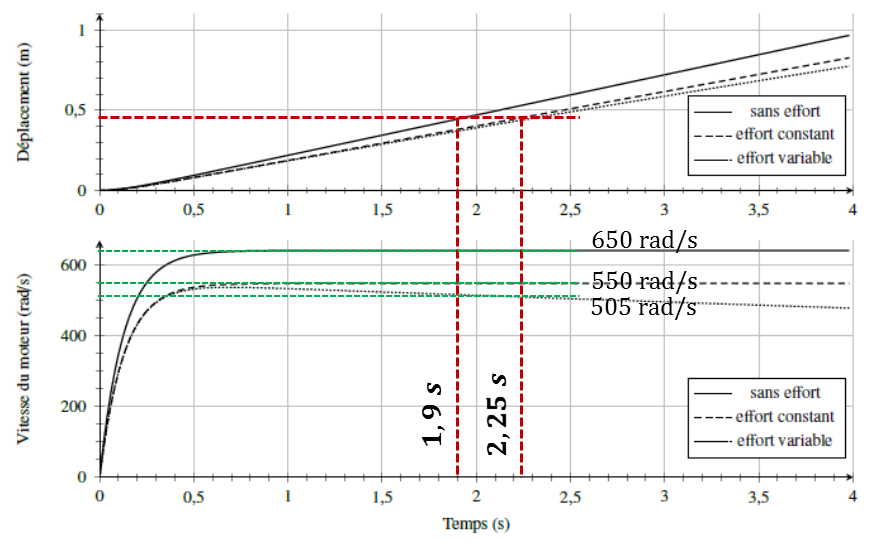
\includegraphics[width=0.9\linewidth]{img/figure11_cor}
\end{center}

Sans effort résistant, le temps de déplacement est de $1.9s$, la vitesse atteinte par le moteur en régime permanent est de $650\ rad.s^{-1}$.

Avec un effort résistant, le temps de déplacement est $2.25s$ de la vitesse atteinte par le moteur en régime permanent est de $550\ rad.s^{-1}$ (effort constant).

Dans les deux cas le cahier des charges est respecté.

Dans les modèles avec prise en compte des frottements la vitesse de rotation du moteur en régime permanent est bien inférieure à celle obtenue sans tenir compte du frottement.

Dans le cas d’un effort variable et à la fin du régime permanent, la vitesse de rotation du moteur est la même que dans le cas précédent puis diminue linéairement au cours du temps.

La prise en compte du frottement avec un effort variable dans la modélisation présente une influence non négligeable et il est préférable d’en tenir compte.}

\reponse{5}{}{
\begin{center}
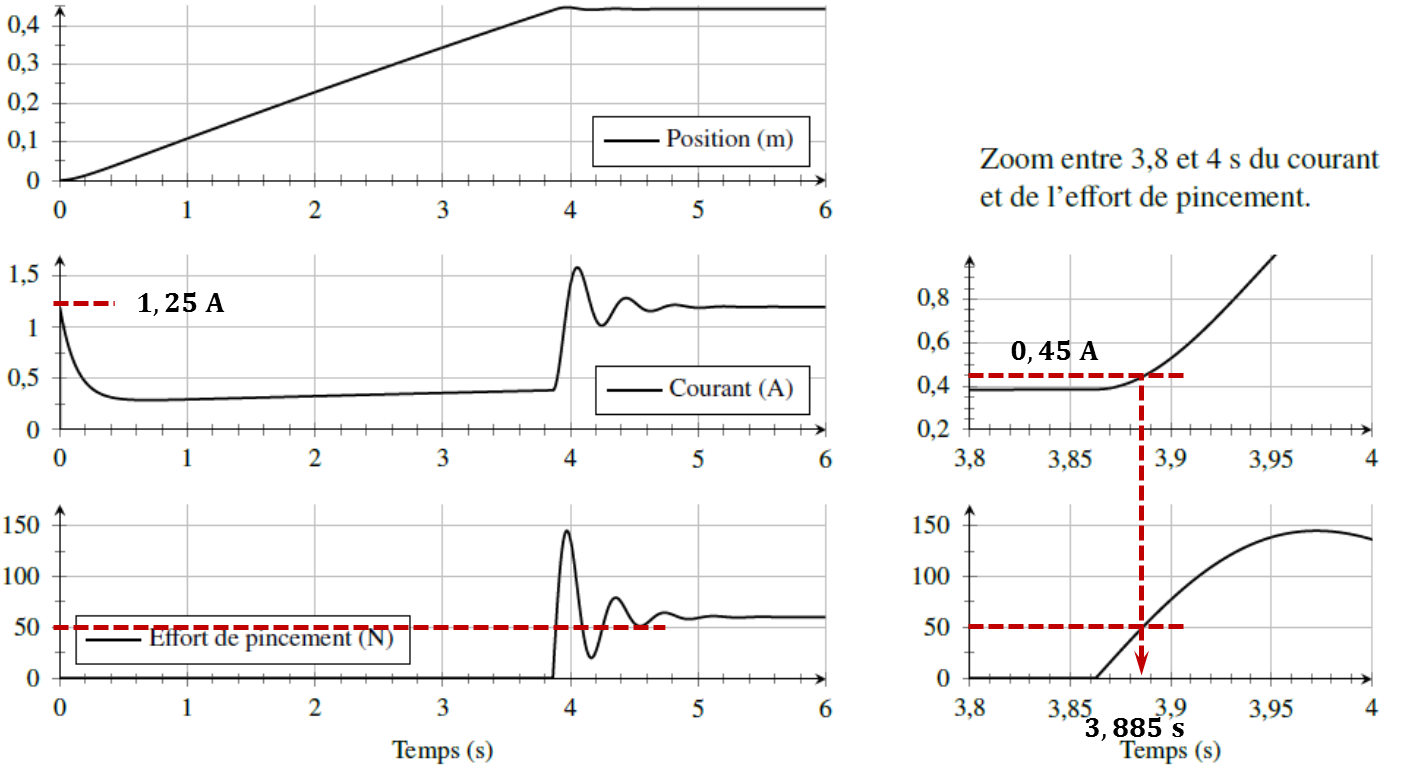
\includegraphics[width=0.9\linewidth]{img/figure12_cor}
\end{center}

L’effort reste inférieur à celui de la législation pendant $3,885\ s$. À ce stade le courant consommé est de $0.45\ A$ à comparer à $1.25\ A$ lors du démarrage du moteur. La méthode de détection de l’effort de pincement par la mesure de courant ne semble donc pas adaptée puisque le courant en régime transitoire est plus important que celui mesuré lors d’un pincement. Avec une méthode de seuillage on n’arriverait donc pas à distinguer la phase de démarrage du moteur et le pincement.}

\reponse{3}{}{
$u_m(t)=R\cdot i(t)+e(t)$\\
$e(t)=k_e\cdot \omega_m(t)$\\
$C_m(t)=k_c\cdot i(t)$
}

\reponse{3}{}{
$\frac{\Omega_m(p)}{U_m(p)}=\frac{k_c}{\left(k_e\cdot k_c+R\cdot f_v \right)}\cdot \frac{1}{1+\frac{RJ}{k_e\cdot k_c+R\cdot f_v}\cdot p}$
}

\reponse{2}{}{
$A(p)=E(p)$
}

\reponse{5}{}{
$E(p)=K_{capt}=A(p)$\\
$D(p)=\frac{C_m(p)}{U_m(p)}=\frac{k_c}{R_m}$\\
$M(p)=\frac{1}{J\cdot p+f_v}$\\
$B(p)= C_{corr}(p)$
}


\reponse{4}{}{
$\varepsilon(p)=\Omega_c(p)-\Omega_m(p)$
$\varepsilon(p)\cdot C(p)=C_m(p)$
or $\left(\Omega_c(p)-\Omega_m(p)\right)\cdot E(p)\cdot B(p)\cdot D(p)=C_m(p)$, donc par identification, on obtient $C(p)=E(p) \cdot B(p) \cdot D(p)$.
}

\reponse{4}{}{
$\begin{cases}
H_1(p)=\frac{C(p) \cdot M(p)}{1+C(p) \cdot M(p)}\\
H_2(p)=-\frac{M(p)}{1+C(p) \cdot M(p)}
\end{cases}$
}

\reponse{8}{}{
$\varepsilon(p)=\Omega_c(p)-\Omega_m(p)$ \\
$\varepsilon(p)=\Omega_c(p)-\left[ \varepsilon(p).C(p)-C_r(p) \right] \cdot M(p)$\\
$\left[ \varepsilon(p).C(p)-C_r(p) \right] \cdot M(p)=\Omega_c(p)-\varepsilon(p)$\\
$\varepsilon(p).(1+C(p)M(p))=\Omega_c(p)+C_r(p)M(p)$\\
$\varepsilon(p)=\frac{\Omega_c(p)+C_r(p)M(p)}{1+C(p)M(p)}=\frac{\Omega_c(p)}{1+C(p)M(p)}+\frac{C_r(p)M(p)}{1+C(p)M(p)} $ \\
$\begin{cases}
  H_c(p)=\frac{1}{1+C(p)M(p)} \\ 
  H_r(p)=\frac{M(p)}{1+C(p)M(p)} 
\end{cases}$
}

\reponse{6}{}{
$\begin{cases}
	H_1(p)=\frac{C(p) \cdot M(p)}{1+C(p) \cdot M(p)}=\frac{K_p\cdot \frac{K}{1+\tau.p}}{1+K_p \cdot \frac{K}{1+\tau.p}}\\
	H_1(p)=\frac{K_p .K}{1+\tau p + K_p.K} \\
	H_1(p)=\frac{K_p.K}{1+K_p.K}\cdot \frac{1}{1+\frac{\tau.p}{1+K_p.K}}
\end{cases}$
Ordre 1, classe 0
}

\reponse{5}{}{
$\begin{cases}
	\omega_m(t)=K’(1-e^{\frac{-t}{\tau’}}) \\
	avec\;K’=\frac{K_p.K}{1+K_p.K}\approx 0.97\;et\;\tau’=\frac{\tau}{1+K_p.K}\approx0.0045s
\end{cases}$
}

\reponse{3}{\begin{center}
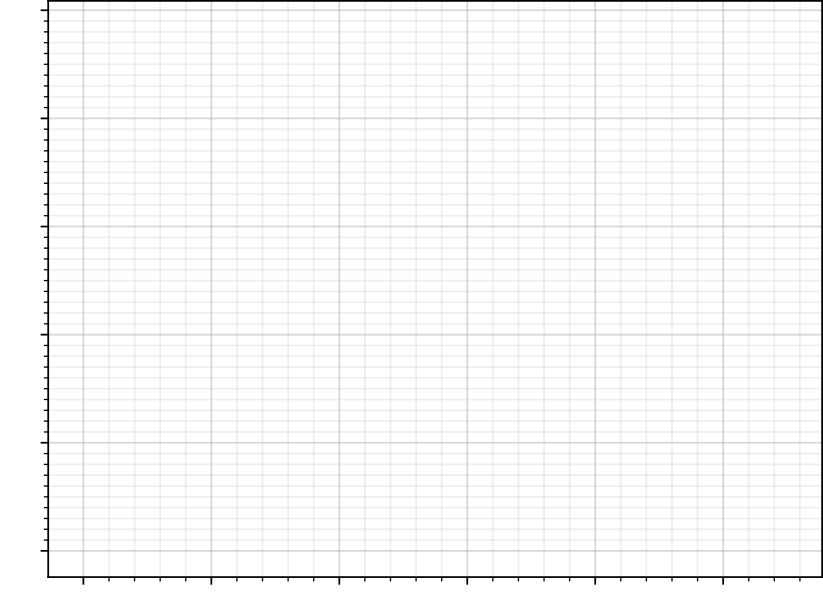
\includegraphics[width=0.8\linewidth]{img/DR21}
\end{center}}{
\begin{center}
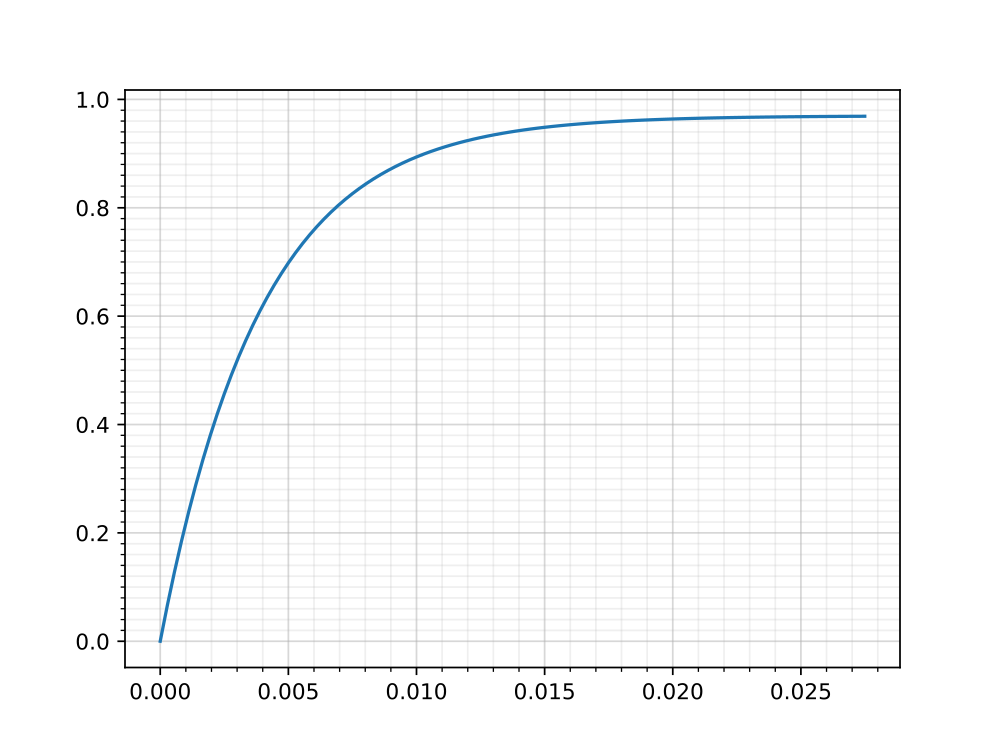
\includegraphics[width=0.8\linewidth]{img/DR21_cor}
\end{center}}

\reponse{5}{}{
$\varepsilon_s=\lim\limits_{t \to \infty}\varepsilon(t)=\lim\limits_{p \to 0}p\cdot \varepsilon(p)$\\
$\varepsilon_s=\lim\limits_{p \to 0}p\cdot \frac{\Omega_c(p)}{1+C(p)M(p)}$\\
$\varepsilon_s=\lim\limits_{p \to 0}p\cdot \frac{\frac{1}{p}}{1+K_p.\frac{K}{1+\tau p}}$\\
$\varepsilon_s=\lim\limits_{p \to 0}\frac{1}{1+K_p.\frac{K}{1+\tau p}}$\\
$\varepsilon_s=\frac{1}{1+K_p.K}\approx 0.03rad.s^{-1}$ \\
On peut également partir de la fonction temporelle $\varepsilon_s=\lim\limits_{t \to \infty}(\Omega_c(t)-\Omega_m(t))$}

\reponse{3}{\begin{center}
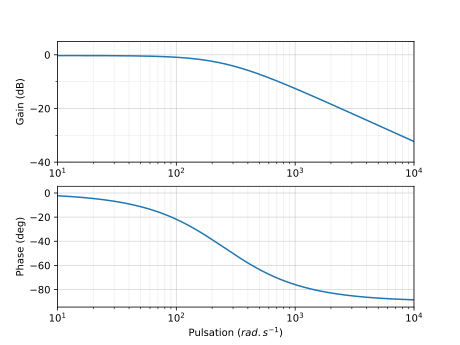
\includegraphics[width=0.85\linewidth]{img/DR23}
\end{center}}{
\begin{center}
$\omega_0\approx 250rad.s^{-1}$\\
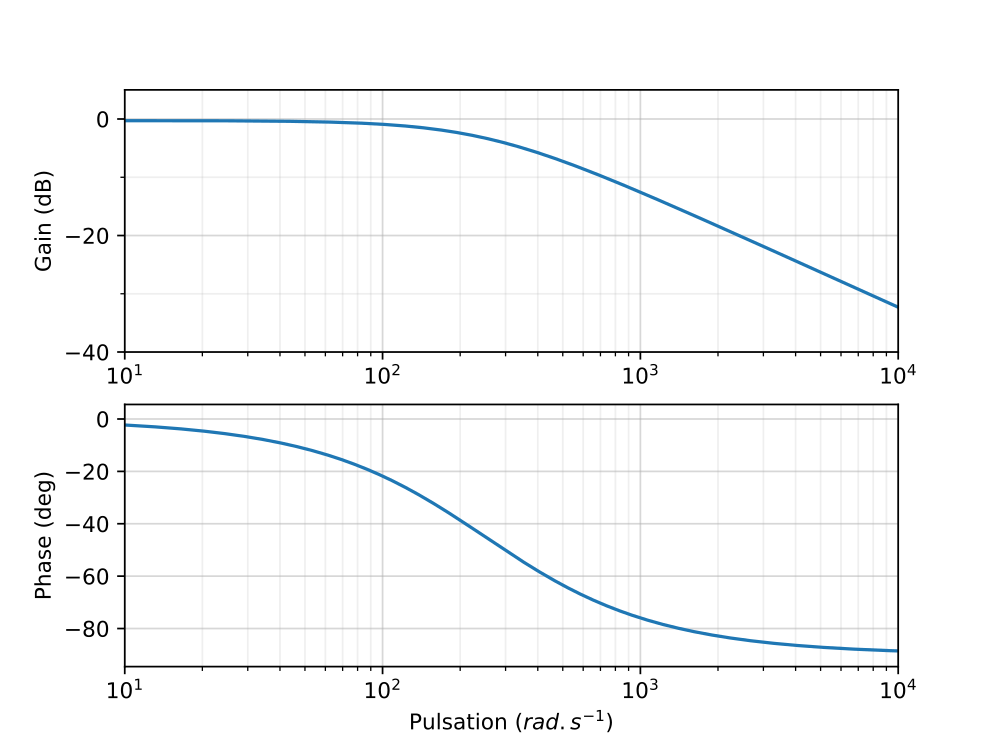
\includegraphics[width=0.85\linewidth]{img/DR23_cor}
\end{center}}


\reponse{6}{}{
$H_1(p)=\frac{C(p) \cdot M(p)}{1+C(p) \cdot M(p)}$\\
$H_1(p)=\frac{K_p\frac{1+\tau_i\;p}{\tau_i\;p} \cdot \frac{K}{1+\tau\;p}}{1+K_p\frac{1+\tau_i\;p}{\tau_i\;p} \cdot \frac{K}{1+\tau\;p}}$\\
$H_1(p)=\frac{K_p\cdot K\cdot (1+\tau_i\;p)}{\tau_i\cdot p\cdot(1+\tau p)+K_p(1+\tau_i\;p)K}$\\
$H_1(p)=\frac{1+\tau_i\;p}{1+\tau_i\cdot(1+\frac{1}{K_pK})\cdot p+\frac{\tau_i \tau}{K_pK} \cdot p^2 }$
ordre 2 classe 0}

\reponse{4}{}{
$\varepsilon_{s1}=\lim\limits_{p \to 0} p\cdot \varepsilon(p)=\lim\limits_{p \to 0} p\cdot\frac{\Omega_c(p)}{1+C(p)M(p)}=\lim\limits_{p \to 0} p\cdot\frac{\frac{\Omega_{c0}}{p}}{1+K_p\frac{1+\tau_i\;p}{\tau_i\;p} \cdot \frac{K}{1+\tau\;p}}$\\
$\varepsilon_{s1}=0$}

\reponse{4}{}{
$\varepsilon_{s2}=\lim\limits_{p \to 0}p\cdot \varepsilon(p)=\lim\limits_{p \to 0}p\cdot\frac{C_r(p)M(p)}{1+C(p)M(p)}=\lim\limits_{p \to 0}p\cdot\frac{\frac{C_{r0}}{p}\cdot \frac{K}{1+\tau\;p}}{1+K_p\frac{1+\tau_i\;p}{\tau_i\;p} \cdot \frac{K}{1+\tau\;p}}$ \\
$\varepsilon_{s2}=\lim\limits_{p \to 0}\frac{C_{r0}\cdot K}{1+K_p\frac{1}{\tau_i\;p} \cdot K}=0$}


\reponse{4}{}{
$\varepsilon_{t1}=\lim\limits_{p \to 0} p\cdot \varepsilon(p)=\lim\limits_{p \to 0} p\cdot\frac{\Omega_c(p)}{1+C(p)M(p)}=\lim\limits_{p \to 0} p\cdot\frac{\frac{\Omega_{c0}}{p^2}}{1+K_p\frac{1+\tau_i\;p}{\tau_i\;p} \cdot \frac{K}{1+\tau\;p}}
=\lim\limits_{p \to 0} p\cdot\frac{\frac{\Omega_{c0}}{p^2}}{\frac{K_p}{\tau_i\;p} \cdot K}$\\
$\varepsilon_{t1}=\frac{\Omega_{c0}\;\tau_i}{K_p\;K}$}

\reponse{4}{}{
$\varepsilon_{t2}=\lim_{p \to 0}p\cdot \varepsilon(p)=\lim\limits_{p \to 0}p\cdot\frac{C_r(p)M(p)}{1+C(p)M(p)}=\lim\limits_{p \to 0}p\cdot\frac{\frac{C_{r0}}{p^2}\cdot \frac{K}{1+\tau\;p}}{1+K_p\frac{1+\tau_i\;p}{\tau_i\;p} \cdot \frac{K}{1+\tau\;p}}$ \\
$\varepsilon_{t2}=\lim\limits_{p \to 0}\frac{1}{p}\;\frac{C_{r0}\cdot K}{1+K_p\frac{1}{\tau_i\;p}\cdot K}=\frac{C_{r0}}{K_p}$}

\reponse{1}{\begin{center}
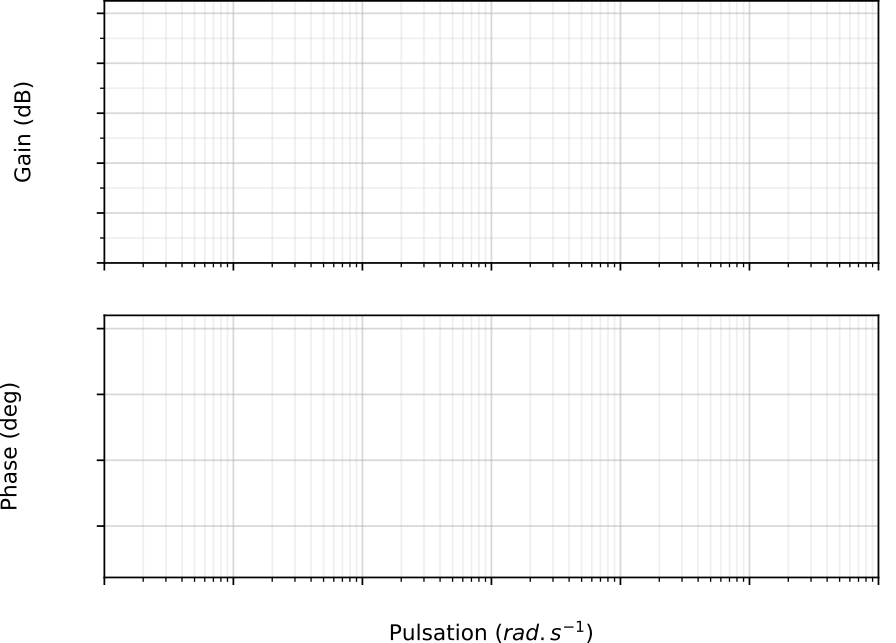
\includegraphics[width=0.8\linewidth]{img/DR29}
\end{center}}{
\begin{center}
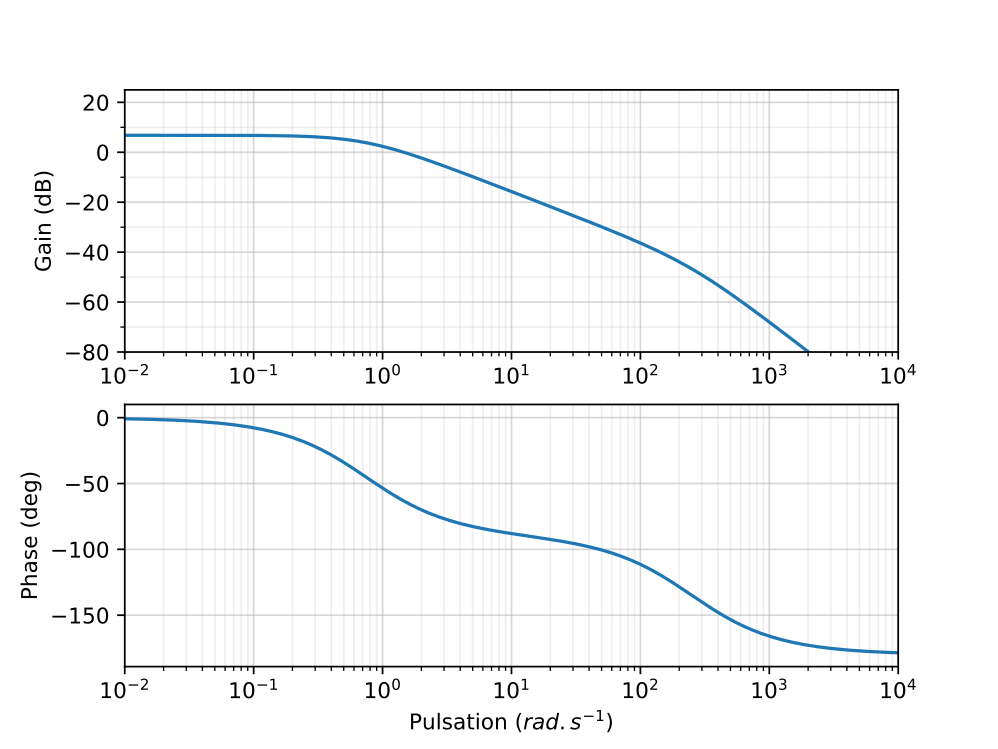
\includegraphics[width=0.8\linewidth]{img/DR29_cor}
\end{center}}

\reponse{1}{\begin{center}
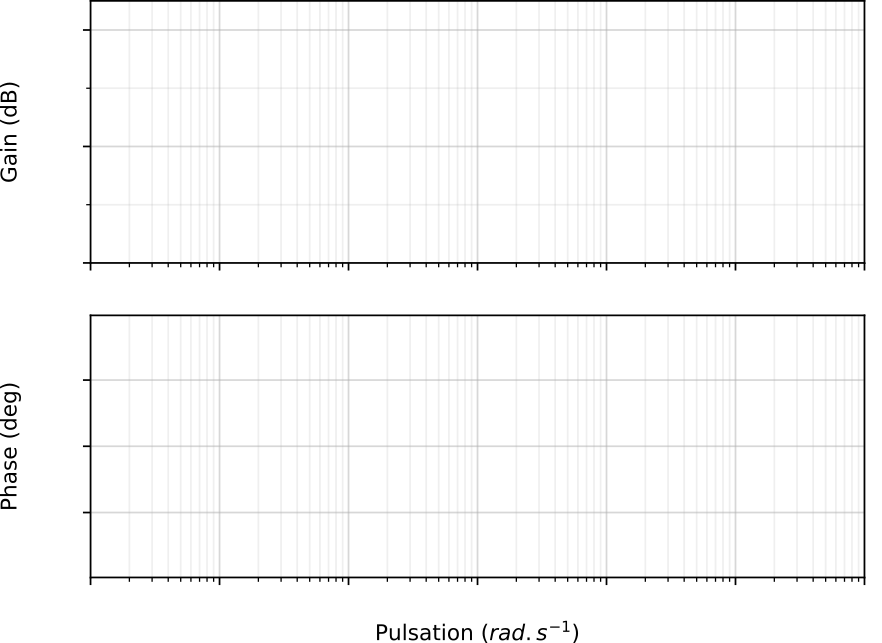
\includegraphics[width=0.8\linewidth]{img/DR30}
\end{center}}{
\begin{center}
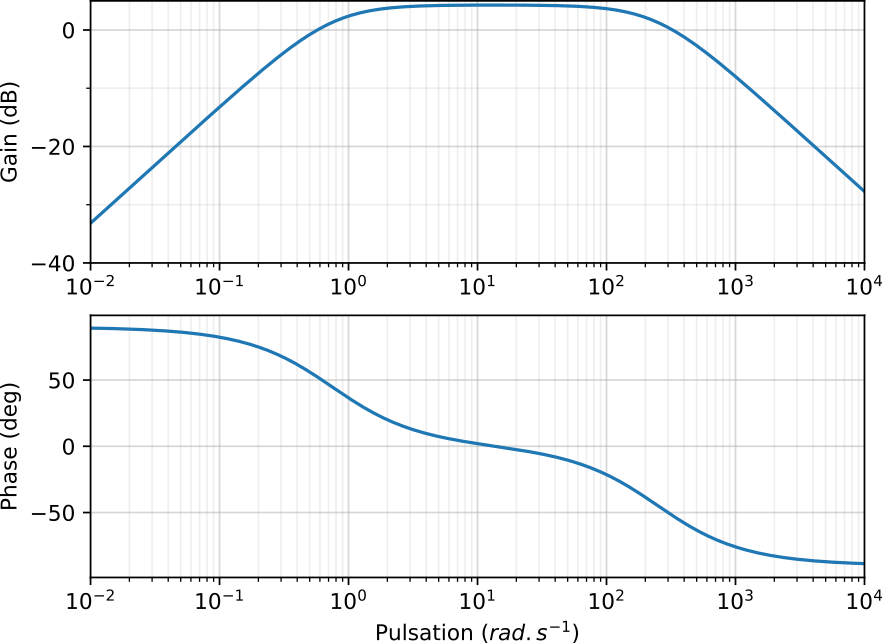
\includegraphics[width=0.8\linewidth]{img/DR30_cor}
\end{center}}

\reponse{6}{}{
Pour $\omega>100rad.s^{-1}$, on peut l'assymiler à un premier ordre de fonction de transfert $H_r(p)=\frac{2.2\cdot p}{1+1.34\cdot p}$

$C_{obs}(p)=\left(\varepsilon(p)-\varepsilon_{t2}\right)\cdot \frac{1+M(p).C(p)}{M(p)}=\left(\varepsilon(p)-\varepsilon_{t2}\right)\cdot \frac{1+\frac{K}{1+\tau p}.K_p\frac{1+\tau_i\cdot p}{\tau_i\cdot p}}{\frac{K}{1+\tau p}}=\left(\varepsilon(p)-\varepsilon_{t2}\right)\cdot \frac{1+\tau p+K.K_p\frac{1+\tau_i\cdot p}{\tau_i\cdot p}}{K}=\left(\varepsilon(p)-\varepsilon_{t2}\right)\cdot \left(\frac{1}{K}+K_p+\frac{\tau}{K}\cdot p+\frac{K_p}{\tau_i\cdot p}\right)$
}


\reponse{6}{}{
L'obstacle apparaît à 5.1s. Il faudrait un seuil pour le détecter.

}

\ifdef{\public}{\newpage}

\reponse{8}{\begin{figure}[!h]
\centering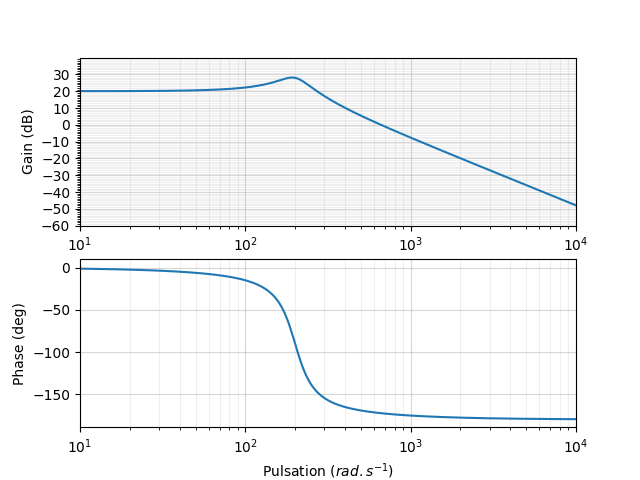
\includegraphics[width=0.9\linewidth]{img/Q33}
 \caption{Diagramme de Bode de la fonction de transfert à identifier}
 \label{img18}
\end{figure}}{

$20\cdot log(K)=20$, donc $K=10$

$20\cdot log\;H_{max}=28$, donc $H_{max}=10^\frac{28}{20}\approx 10^\frac{3}{2}=\sqrt{10}^3\approx 27$

$Q=\frac{H_{max}}{H(0)}=2.7=\frac{1}{2\cdot \xi \cdot \sqrt{1-\xi^2}}$

$2.7^2=2.7*2+2.7*0.7=5.4+1.9=7.3$ et $\frac{1}{7.3}\approx\frac{1}{7.5}\approx 0.13$
Donc $4\cdot \xi^2 \cdot (1-\xi^2)=0.13$

Soit $X=\xi^2$,

$4\cdot X -4\cdot X^2=0.13$

$X^2-X+0.03=0$

$\Delta=1-0.13=0.87$

$\sqrt{\Delta}=\sqrt{\frac{9}{10}}=\frac{3}{3.14}=\frac{1}{1.05}=1-\frac{0.05}{1.05}=1-\frac{0.05}{1.05}\approx0.94$

$x=\frac{1\pm0.94}{2}$

$x1=0.03$ et $x2=0.97$

Donc $\xi=\sqrt{0.03}\approx0.17$, $\omega_0=200rad.s^{-1}$ et $K=10$.
}


\end{document}

